%%%%%%%%%%%%%%%%%%%%%%%%%%%%%%%%%%%%%%%%%%%%%%%%%%%%%%%%%%%%%%%%%%%%%%%%%%%%%%%%
%%%%%%%%%%%%%%%%%%%%%%%%%%%%%%%%%%%%%%%%%%%%%%%%%%%%%%%%%%%%%%%%%%%%%%%%%%%%%%%%
%
% A general frame for lecture slides and lecture notes in one file
% using LaTeX beamer
%
%%%%%%%%%%%%%%%%%%%%%%%%%%%%%%%%%%%%%%%%%%%%%%%%%%%%%%%%%%%%%%%%%%%%%%%%%%%%%%%%
%%%%%%%%%%%%%%%%%%%%%%%%%%%%%%%%%%%%%%%%%%%%%%%%%%%%%%%%%%%%%%%%%%%%%%%%%%%%%%%%

% only for the article version
\mode<article> 
{
  \usepackage[automark,komastyle]{scrpage2}
  \usepackage{amsfonts}
  \usepackage{amsthm}
  \usepackage{amscd}
  \usepackage{fullpage}
  \setlength{\parindent}{0pt}
  \setlength{\parskip}{1.25ex plus 0.5ex minus 0.2ex}
}

% only presentation 
\mode<presentation>
{
%  \usepackage{times}
%  \usetheme{default}
  \usetheme[secheader]{Boadilla}
  \setbeamercovered{transparent}
  \setbeamertemplate{background canvas}[vertical shading][bottom=white!10,top=white!10]
  \setlength{\parindent}{0pt}
  \setlength{\parskip}{1.35ex plus 0.5ex minus 0.3ex}
  \setbeamertemplate{theorems}[numbered]
  \usefonttheme[onlysmall]{structurebold}
  \usepackage{amscd}
}

% all after
\usepackage{graphicx}
%\usepackage{multimedia}
\usepackage{psfrag}
\usepackage{listings}
\lstset{language=C++, basicstyle=\ttfamily, 
  keywordstyle=\color{black}\bfseries, tabsize=4, stringstyle=\ttfamily,
  commentstyle=\it, extendedchars=true, escapeinside={/*@}{@*/}}
\usepackage{curves}
%\usepackage{epic}
\usepackage{calc}
\usepackage{picinpar}
%\usepackage{fancybox}
%\usepackage{xspace}
\usepackage{enumerate}
\usepackage{algorithmic}
\usepackage{algorithm}
\usepackage{bm}

\mode<article> 
{
\usepackage{hyperref}
}

%The theorems
\mode<article> 
{
\newtheoremstyle{mystyle}%
{3pt}%
{3pt}%
{}%
{}%
{\sffamily\bfseries}%
{.}%
{.5em}%
{}%
\theoremstyle{mystyle}
}
\mode<presentation> 
{
\theoremstyle{definition}
}
\newtheorem{Def}{Definition}%[section]
\newtheorem{Exm}[Def]{Example}
\newtheorem{Lem}[Def]{Lemma}
\newtheorem{Rem}[Def]{Remark}
\newtheorem{Rul}[Def]{Rule}
\newtheorem{Thm}[Def]{Theorem}
\newtheorem{Cor}[Def]{Corollary}
\newtheorem{Obs}[Def]{Observation}
\newtheorem{Ass}[Def]{Assumption}
\newtheorem{Pro}[Def]{Property}
\newtheorem{Alg}[Def]{Algorithm}
\newtheorem{Prp}[Def]{Proposition}
\newtheorem{Lst}[Def]{Listing}

% Delete this, if you do not want the table of contents to pop up at
% the beginning of each subsection:
\AtBeginSection[]
{
  \begin{frame}<beamer>
    \frametitle{Contents}
\tableofcontents[currentsection,sectionstyle=show/hide,subsectionstyle=show/show/hide]
%    \tableofcontents[currentsection]
  \end{frame}
}

% Title definition
\mode<presentation>
{
  \title{\texttt{dune-pdelab} Howto}
  \author{Peter Bastian}
  \institute[IWR]
  {
    Universit�t Heidelberg\\
    Interdisziplin�res Zentrum f�r Wissenschaftliches Rechnen\\
    Im Neuenheimer Feld 368, D-69120 Heidelberg\\
	email: \url{Peter.Bastian@iwr.uni-stuttgart.de}
  }
  \date{\today}
  \logo{\includegraphics[width=9mm]{./EPS/iwrlogo-klein.eps}}
}
\mode<article>
{
  \title{\texttt{dune-pdelab} Howto}
  \author{\textsc{Peter Bastian}\\
    Universit�t Heidelberg\\
    Interdisziplin�res Zentrum f�r Wissenschaftliches Rechnen\\
    Im Neuenheimer Feld 368, D-69120 Heidelberg\\
	email: \url{Peter.Bastian@iwr.uni-stuttgart.de}
  }
  \date{\today}
  \publishers{%
  \vspace{10mm}
  \includegraphics[width=0.9\textwidth]{./EPS/rotbilinear}
  \\
  \vspace{10mm}
  \url{http://www.dune-project.org/}\\
  }
}

% logo nach oben
\mode<presentation>
{
% No navigation symbols and no lower logo
\setbeamertemplate{sidebar right}{}

% logo
\newsavebox{\logobox}
\sbox{\logobox}{%
    \hskip\paperwidth%
    \rlap{%
      % putting the logo should not change the vertical possition
      \vbox to 0pt{%
        \vskip-\paperheight%
        \vskip0.35cm%
        \llap{\insertlogo\hskip0.1cm}%
        % avoid overfull \vbox messages
        \vss%
      }%
    }%
}

\addtobeamertemplate{footline}{}{%
    \usebox{\logobox}%
}
}

% number equations within sections in article mode
%\numberwithin{equation}{section}

% math symbols
\newcommand{\diffd}{\,d}

%%%%%%%%%%%%%%%%%%%%%%%%%%%%%%%%%%%%%%%%%%%%%%%%%%%%%%%%%%%%%%%%%%%%%%%%%%%%%%%%
%%%%%%%%%%%%%%%%%%%%%%%%%%%%%%%%%%%%%%%%%%%%%%%%%%%%%%%%%%%%%%%%%%%%%%%%%%%%%%%%
%
% now comes the individual stuff lecture by lecture
%
%%%%%%%%%%%%%%%%%%%%%%%%%%%%%%%%%%%%%%%%%%%%%%%%%%%%%%%%%%%%%%%%%%%%%%%%%%%%%%%%
%%%%%%%%%%%%%%%%%%%%%%%%%%%%%%%%%%%%%%%%%%%%%%%%%%%%%%%%%%%%%%%%%%%%%%%%%%%%%%%%
\mode<article>
{
\pagestyle{scrheadings}
}

\begin{document}

\mode<presentation>
{
  \begin{frame}
    \titlepage
  \end{frame}
}
\mode<article>
{
\maketitle
}

\begin{abstract}
This article contains concepts for a general discretization module for
the ``Distributed Numerics Environment'' DUNE \cite{Dune2008a,Dune2008b}. It should enable one
to build up a library of finite element methods in an easy and
extendable way that is closely related to the mathematical formulation
of finite element methods. 
\end{abstract}

\mode<article>
{
\cleardoublepage
}

\mode<presentation>{
\begin{frame}<presentation>
\frametitle{Outline}
\tableofcontents[section,sectionstyle=show/show,subsectionstyle=hide/hide/hide] 
\end{frame}
}

\mode<article>
{
\tableofcontents
}

\mode<article>
{
\cleardoublepage
}

%%%%%%%%%%%%%%%%%%%%%%%%%%%%%%%%%%%%%%%%%%%%%%%%%%%%%%%%%%%%
%%%%%%%%%%%%%%%%%%%%%%%%%%%%%%%%%%%%%%%%%%%%%%%%%%%%%%%%%%%%
%%%%%%%%%%%%%%%%%%%%%%%%%%%%%%%%%%%%%%%%%%%%%%%%%%%%%%%%%%%%
\section{Introduction}
%%%%%%%%%%%%%%%%%%%%%%%%%%%%%%%%%%%%%%%%%%%%%%%%%%%%%%%%%%%%
%%%%%%%%%%%%%%%%%%%%%%%%%%%%%%%%%%%%%%%%%%%%%%%%%%%%%%%%%%%%
%%%%%%%%%%%%%%%%%%%%%%%%%%%%%%%%%%%%%%%%%%%%%%%%%%%%%%%%%%%%

\subsection{PDELab Aims and Features}

\begin{frame}
\frametitle<presentation>{DUNE PDELab Features}
\begin{itemize}
\item Rapid prototyping: Substantially reduce time to implement
discretizations and solvers for systems of PDEs based on DUNE.
\item Simple things should be simple --- suitable for teaching.
\item Discrete function spaces spaces:
\begin{itemize}
\item Conforming and non-conforming,
\item hp-refinement,
\item general approach to constraints,
\item generic generation of product spaces for systems.
\end{itemize} 
\item Operators based on weighted residual formulation:
\begin{itemize}
\item Linear and nonlinear,
\item stationary and transient,
\item FE and FV schemes requiring at most face-neighbors.
\end{itemize} 
\item Exchangeable linear algebra backend. 
\item User only involved with ``local'' view on (reference) element.
\end{itemize}
\end{frame}

\begin{frame}
\frametitle<presentation>{DUNE Module Architecture}
Major DUNE modules are:
\begin{center}
\mode<presentation>{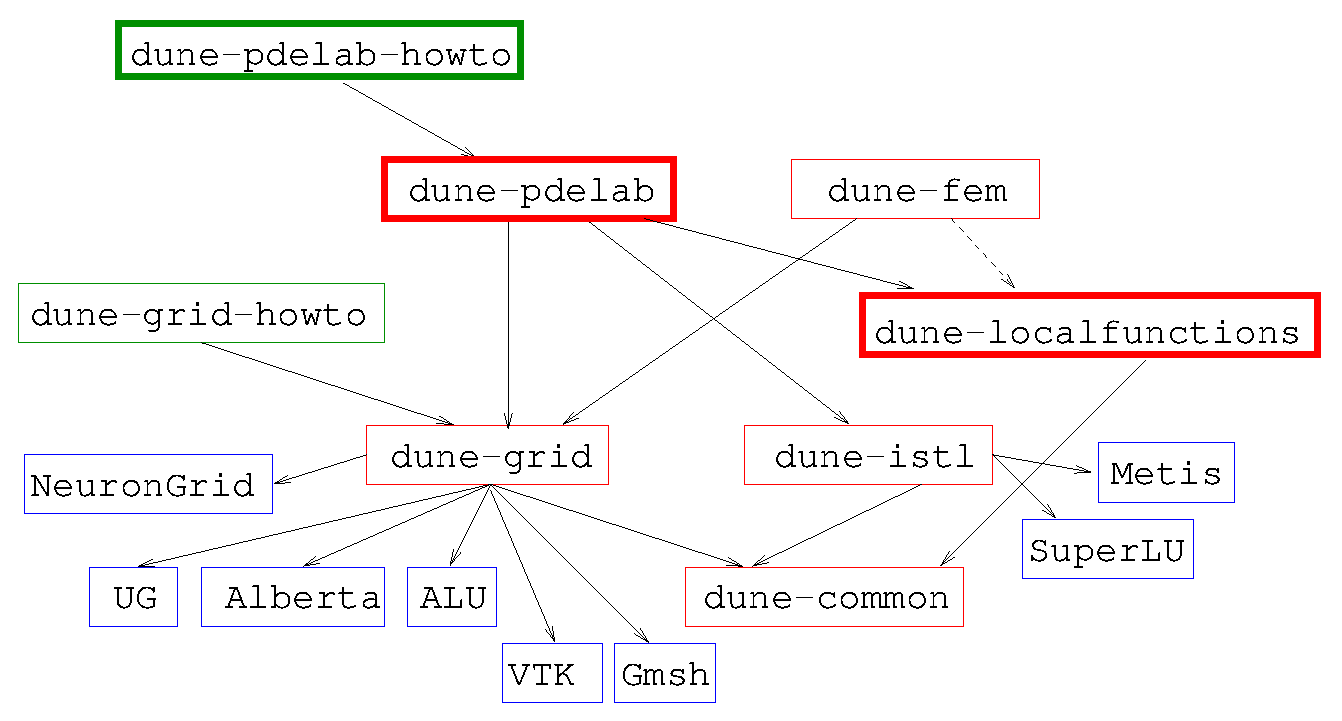
\includegraphics[width=1.0\textwidth]{./EPS/modules.eps}}
\mode<article>{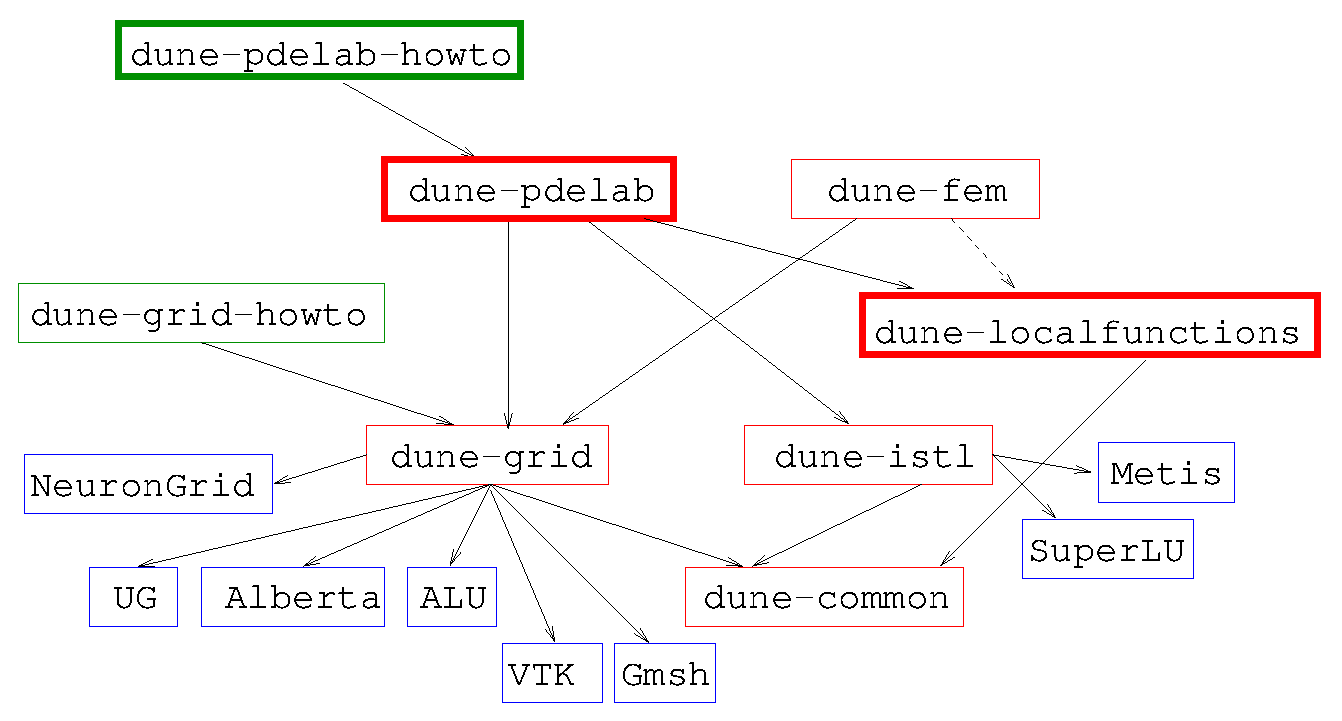
\includegraphics[width=0.7\textwidth]{./EPS/modules.eps}}
\end{center}
\end{frame}

\begin{frame}
\frametitle<presentation>{Required Modules}
To work through the examples the following DUNE modules are required: 
\begin{itemize}
\item \lstinline{dune-common},
\item \lstinline{dune-grid},
\item \lstinline{dune-istl},
\item \lstinline{dune-localfunctions},
\item \lstinline{dune-pdelab},
\item \lstinline{dune-pdelab-howto},
\end{itemize}

In addition, at least one of the grid managers UG, ALU or Alberta is
required to do the examples on simplex grids. 
\end{frame}



\subsection{How to Read this Manual}

Section 2 introduces the \textit{weighted residual formulation} which
is the abstract formulation of PDE problems in PDELab. You should at
least get some idea about it on your first reading.

Section 3 presents the theory behind grid function
spaces including the constuction of subspaces due to general
constraints. An understanding of this is necessary if you want to
implement new function spaces or constraints.

Section 4 provides a step by step introduction to the implementation
of grid function spaces. Working through these examples will enable
you to use existing function spaces and implement new ones.

Section 5 contains the theory behind the solution of the algebraic
systems arising from the constrained weigthed residual formulation.

Section 6 then shows how a discretization scheme is implemented using
the grid function spaces. A simple conforming discretization of the
Laplacian is worked through in detail and the set-up of solvers
using \lstinline{dune-istl} is explained.

Section 7 contains a list of the problems implemented in
the \lstinline{examples} directory.

\cleardoublepage

%%%%%%%%%%%%%%%%%%%%%%%%%%%%%%%%%%%%%%%%%%%%%%%%%%%%%%%%%%%%
%%%%%%%%%%%%%%%%%%%%%%%%%%%%%%%%%%%%%%%%%%%%%%%%%%%%%%%%%%%%
%%%%%%%%%%%%%%%%%%%%%%%%%%%%%%%%%%%%%%%%%%%%%%%%%%%%%%%%%%%%
\section{Weighted Residual Formulation}
%%%%%%%%%%%%%%%%%%%%%%%%%%%%%%%%%%%%%%%%%%%%%%%%%%%%%%%%%%%%
%%%%%%%%%%%%%%%%%%%%%%%%%%%%%%%%%%%%%%%%%%%%%%%%%%%%%%%%%%%%
%%%%%%%%%%%%%%%%%%%%%%%%%%%%%%%%%%%%%%%%%%%%%%%%%%%%%%%%%%%%

\subsection{Abstract Formulation}

When we go about to solve a PDE problem we need a general idea of what
a PDE problem is. We will develop such an idea in this section.

\begin{frame}
\frametitle<presentation>{Weighted Residual Formulation}
\begin{Def}[Weighted Residual Formulation]
We claim that all problems we ever want to solve can be written in the form
\begin{equation}
\text{Find } u_h\in w_h + \tilde{U}_h : \qquad r_h(u_h,v) =
0 \qquad \forall v\in \tilde{V}_h.  
\end{equation}
Where:
\begin{itemize}
\item $\tilde{U}_h\subseteq U_h$, $\tilde{V}_h\subseteq V_h$ are
finite-dimensional function spaces and corresponding subspaces.
\item Affine shift: $u_h\in w_h + \tilde{U}_h$ for a given $w_h\in U_h$ means
$u_h = w_h + \tilde{u}_h$ for some $\tilde{u}_h\in\tilde{U}_h$.
\item $r_h : U_h \times V_h \to \mathbb{K}$ is the \textit{residual form}.
\begin{itemize}
\item $r_h$ may be \textit{nonlinear} in its first argument.
\item $r_h$ \textit{is always linear} in its second argument.
\item $r_h$ may depend on the grid in non-conforming methods.
\end{itemize}
\item We assume that this problem has a unique solution. \hfill$\square$
\end{itemize}
\end{Def}
\end{frame}

We now give some concrete examples.

\subsection{Some Examples}

\paragraph{Continuous Problem}

\begin{frame}
\frametitle<presentation>{Continuous Problem}

Consider the Poisson equation
\begin{subequations}
\label{Eq:DiffusionEquation}
\begin{align}
                -\Delta u &= f& \text{in }& \Omega\subseteq\mathbb{R}^n,\\
                        u &= g& \text{on }& \Gamma_D\subseteq\partial\Omega,\\
     - \nabla u\cdot\nu   &= j& \text{on }& \Gamma_N=\partial\Omega\setminus\Gamma_D,
\end{align}
\end{subequations}
where $\mbox{meas}(\Gamma_D)\neq 0$. 

The \textit{weak formulation} uses the spaces
\begin{equation*}
U = H^1(\Omega), \qquad
\tilde{U} = \{u \in U\,|\, \text{``$u=0$'' on $\Gamma_D$}
\}
\end{equation*}
and reads
\begin{equation}\label{Eq:DiffusionWeakForm}
u \in w+\tilde{U} \  : \quad
\underbrace{\int_\Omega \nabla u \cdot \nabla v \diffd x
+ \int_{\Gamma_N} j v \diffd s - \int_\Omega f v \,dx}_{= r(u,v)} = 0,  
\quad \forall v\in \tilde{U}.
\end{equation}
Here $w\in U$ is a function with ``$w=g$'' on $\Gamma_D$ and $V=U$, $\tilde{V}=\tilde{U}$.
\end{frame}


\paragraph{Conforming Finite Elements of Order $k$}

First we need to introduce some notation for the grid:

\begin{frame}
\frametitle<presentation>{Conforming Finite Elements of Order $k$}
$\mathbb{T}_h$ is a grid with elements
$E_h^0=\{e_0,\ldots,e_{N_h^0-1}\}$
covering the domain $\Omega\subset\mathbb{R}^n$.

$\Omega_e$ is the domain (open, connected set) associated with element
$e\in E_h^0$.

The discrete function spaces now are
\begin{align*}
U_h^k &= \{u\in C^0(\Omega) \,|\, u|_{\Omega_e}\in P_k
\}, &
\tilde{U}_h^k &= \{u \in U_h^k \,|\, \text{``$u(x) = 0$'' for $x\in\Gamma_D$}\}.
\end{align*}
$P_k$ are the polynomials of degree $k$ and $\Gamma_D$ is resolved
by the mesh.

Now take $w_h\in U_h^k$ with ``$w_h(x) = g(x)$'' (sample at vertices)
on $\Gamma_D$ and find $u_h\in w_h+\tilde{U}_h^k$ s.t.  
\begin{equation}
\underbrace{\int_\Omega \nabla u_h \cdot \nabla v \diffd x
+ \int_{\Gamma_N} j v \diffd s - \int_\Omega f v \,dx}_{= r^\text{FE}_h(u,v)}
 = 0 \qquad \forall v\in \tilde{U}^k_h.
\end{equation}
Obviously, we have $r^\text{FE}_h(u_h,v) = r(u_h,v)$.
\end{frame}

\paragraph{Vertex-centered Finite Volumes}

This method uses a discontinuous test space that is constant on
``cells''. Let us introduce some notation to define this formally.

\begin{frame}
\frametitle<presentation>{Vertex-centered Finite Volumes}
\begin{window}[0,r,{
\psfrag{bi}{$c_i$}
\psfrag{vi}{$z_i$}
\psfrag{bj}{$c_j$}
\psfrag{vj}{$z_j$}
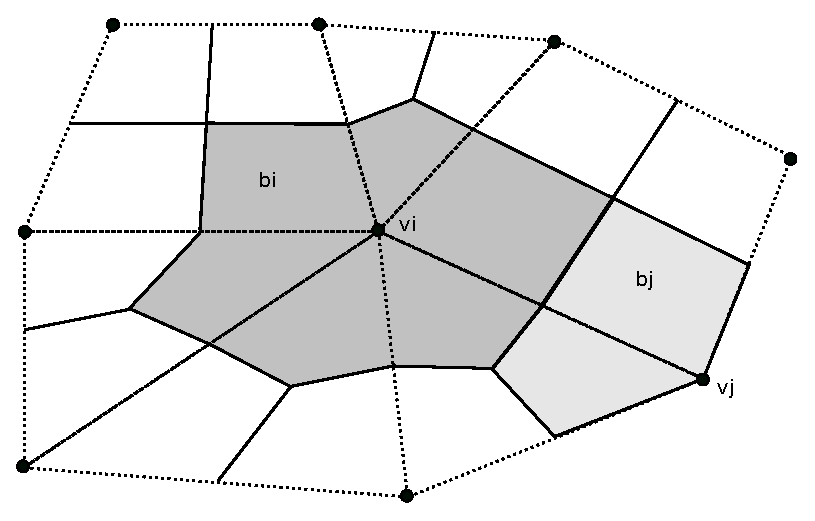
\includegraphics[width=0.4\textwidth]{./EPS/SecMesh2D.eps}},{}]
$E_h^d=\{z_0,\ldots,z_{N_h^d-1}\}$ are the vertices of the mesh
(entities of codimension $d$). 

$x_z$ is the position of $z\in E_h^d$.

$C_h = \{c_0,\ldots,c_{N_h^d-1}\}$ are ``cells'' around each vertex of
the mesh.
\end{window}

$\Omega_c$ is the domain of $c\in C_h$ and $x_c=x_z$ when $c$ is the
cell around $z$.

Define the \textit{discontinuous} test function space:
\begin{align*}
V_h^0 & = \{ v\in L_2(\Omega) \,|\, \forall c\in C_h : v|_{\Omega_c} =
\text{const} \},\\
\tilde{V}_h^0 &= \{ v\in V_h \,|\, \forall z\in E_h^d, x_z\in\Gamma_D : v(x_z)=0\}.
\end{align*}

\end{frame}

\begin{frame}
\frametitle<presentation>{Vertex Centered Finite Volumes (Contd.)}
The discontinuities are located on the \textit{skeleton} which is given by:
\begin{equation*}
\Gamma_h^{\text{int}} = \{\gamma_{e,c,c^\prime} \,|\,
\gamma_{e,c,c^\prime} = \Omega_e \cap \partial\Omega_c \cap
\partial\Omega_{c^\prime} \}
\end{equation*}
and the boundary faces are given by
\begin{equation*}
\Gamma_h^{\text{ext}} = \{\gamma_{e,c} \,|\,
\gamma_{e,c} = \partial\Omega_e \cap \partial\Omega_c \cap
\partial\Omega \}.
\end{equation*}

For $\gamma\in\Gamma_h^{\text{int}}$, $\nu_\gamma(x)$ is
the \textit{unique} unit
normal vector to $\gamma$ in point $x$. 

Similarly, for
$\gamma\in\Gamma_h^{\text{ext}}$, $\nu_\gamma(x)$ is the unit outer
normal vector.

The jump of a function $v\in V_h$ in
$x\in\gamma\in\Gamma_h^{\text{int}}$ given by
\begin{equation*}
[v]_\gamma(x) = \lim_{\varepsilon\to 0-} v(x+\varepsilon \nu_\gamma(x))
-  \lim_{\varepsilon\to 0+} v(x+\varepsilon \nu_\gamma(x))\quad.
\end{equation*}
\end{frame}

\begin{frame}
\frametitle<presentation>{Vertex Centered Finite Volumes (Contd.)}
The discrete problem then reads as follows. Find $u_h\in w_h+\tilde{U}_h^1$ s.t.
\begin{equation}
\underbrace{- \sum_{\gamma\in\Gamma_h^{\text{int}}} \int_\gamma
\nabla u_h \cdot \nu_\gamma \,[v]\diffd s
+ \sum_{\substack{\gamma\in\Gamma_h^{\text{ext}},\\ \gamma\subseteq\Gamma_N}}
\int_\gamma j v \diffd s\quad
- \int_\Omega fv \diffd x}_{= r_h^\text{FE}(u_h,v)} = 0,
\quad \forall v\in \tilde{V}_h^0.
\end{equation}
$\tilde{U}_h^1$ is the linear conforming finite element space and $w_h$ is
defined as before.

Typically, the integrals are evaluated with low order quadrature rules
such as the midpoint rule.

This gives a simple example with non-conforming residual form and
different trial and test functions.
\end{frame}


\paragraph{Cell Centered Finite Volumes}

\begin{frame}
\frametitle<presentation>{Cell Centered Finite Volumes}
Assume that $\mathbb{T}_h$ is either a Delauney
triangulation or a structured cube mesh.

$E^1_h = \{f_0,\ldots,f_{N^1_h-1}\}$ is the set of interior
faces (intersections of two \textit{elements}).

$B^1_h = \{b_0,\ldots,b_{NB^1_h-1}\}$ is the set of exterior faces
(intersections of elements with the domain boundary).

$l,r : E^1_h \to E^0_h$ deliver the ``left'' and ``right'' elements for an
interior face. 

$\nu_f$ denotes the unit normal vector to $f\in E^1_h$ that points from
$l(f)$ to $r(f)$.

Similarly, $l : B^1_h \to E^0_h$ gives the element where $b\in B_h$ is a
face of and $\nu_b$ is the unit outer normal.
\end{frame}

%$\Omega_f$ is the domain of $f\in E_h^1, B_h^1$, $x_f$ is its center.

%$\omega_e = \text{interior}(\overline{\omega_{l(e)}\cup
%\omega_{r(e)}})$ is the domain of the two elements adjacent to $e\in
%E_h$.

%$\omega_b = \omega_{l(e)}$. 

\begin{frame}
\frametitle<presentation>{Cell Centered Finite Volumes (Contd.)}
Define space of \textit{element-wise} constant functions:
\begin{equation*}
W_h^0 = \{  u\in L_2(\Omega) \,|\, \forall e\in E^0_h : u|_{\Omega_e} =
\text{const} \} .
\end{equation*}

The discrete problem then reads
\begin{equation*}
u_h\in W_h^0 \ : \ r_h^\text{CC}(u_h,v) = 0 \quad \forall v\in W^0_h
\end{equation*}
where
\begin{equation*}
\begin{split}
r_h^\text{CC}(u,v) &= \sum_{f\in E^1_h} \int_{\Omega_f}
\frac{u(x_{l(f)}-u(x_{r(f)}))}{\|x_{r(f)}-x_{l(f)}
\|}\,[v]\diffd s
+ \sum_{\substack{b\in B^1_h\\ \Omega_b\subseteq\Gamma_D}} \int_{\Omega_b}
\frac{u(x_{l(b)}-g(x_b))}{\|x_{b}-x_{l(b)}\|}\, v \diffd s \\
& \qquad - \int_\Omega fv \diffd x -
\sum_{\substack{b\in B^1_h\\ \Omega_b\subseteq\Gamma_N}}
\int_{\Omega_b} j v \diffd s .
\end{split}
\end{equation*}

Note that in this formulation there are no essential boundary
conditions. 
\end{frame}

\paragraph{Discontinuous Galerkin}

\begin{frame}
\frametitle<presentation>{Discontinuous Galerkin Finite Element
Method}
Let $k : E^0_h \to \mathbb{N}_0$ be a function that associates an
nonnegative integer with each element.

Define the discrete function space
\begin{equation*}
W_h^k = \{u\in L_2(\Omega) \,|\, \forall e\in E^0_h : u|_{\Omega_e} \in P_{k(e)}\}.
\end{equation*}

For any $x\in\Omega_f, f\in E_h^1$, define the jump of a function
$u\in W_h^k$:
\begin{equation*}
\label{Eq:Jump}
[u]_f(x) = \lim\limits_{\epsilon\to 0-} u(x+\epsilon\nu_f) - 
\lim\limits_{\epsilon\to 0+} u(x+\epsilon\nu_f).
\end{equation*}

For any $x\in\Omega_f, f\in E_h^1$, define the average of a function
$u\in W_h^k$:
\begin{equation*}
\label{Eq:Average}
\langle u\rangle_f(x) = \frac{1}{2}\left(\lim\limits_{\epsilon\to 0-} u(x+\epsilon
\nu_f) +  \lim\limits_{\epsilon\to 0+} u(x+\epsilon
\nu_f)\right ).
\end{equation*}

\end{frame}


\begin{frame}
\frametitle<presentation>{Discontinuous Galerkin Finite Element
Method (Contd.)}
The discrete problem for the OBB method \cite{OBB98} then reads
\begin{equation*}
u_h \in W^k_h \quad : \quad r_h^\text{OBB}(u_h,v) = 0 \qquad \forall v\in W_h^k,
\end{equation*}
where
\begin{equation*}
\begin{split}
r_h^\text{OBB}(u &,v) = \sum_{e\in E_h^0} \int_{\Omega_e} \nabla u\cdot \nabla v
 - fv \, dx \\
&+ \sum_{f\in E^1_h} \int_{\Omega_f} \langle \nabla v\cdot\nu_f\rangle [u]_f
- [v]_f \langle \nabla u\cdot \nu_f\rangle \, ds\\
&+ \sum_{\substack{b\in B^1_h\\\Omega_b\subseteq\Gamma_D}} \int_{\Omega_b} (\nabla v\cdot\nu_f) (u-g)
- v (\nabla u\cdot \nu_f) \, ds + \sum_{\substack{b\in
B^1_h\\\Omega_b\subseteq\Gamma_N}} \int_{\Omega_b} j v \,ds .
\end{split}
\end{equation*}
Note the seperation into volume, skeleton and boundary terms.
\end{frame}


\paragraph{Crouzeix-Raviart}

\begin{frame}
\frametitle<presentation>{Crouzeix-Raviart Element}
Here we use the following discrete spaces:
\begin{align*}
X_h &= \{u\in L_2(\Omega) \,|\, u|_{\Omega_e}\in P_1 \text{ and $u$
continuous at face centers}\},\\
\tilde{X}_h &= \{u\in X_h \,|\, \text{``$u=0$'' on $\Gamma_D$}\}.
\end{align*}

The discrete problem then reads
\begin{equation*}
u_h \in w_h+\tilde{X}_h \quad : \quad r_h^\text{CR}(u_h,v) = 0 \qquad \forall v\in \tilde{X}_h,
\end{equation*}
where
\begin{equation*}
\begin{split}
r_h^\text{CR}(u &,v) = \sum_{e\in E_h^0} \int_{\Omega_e} \nabla u\cdot \nabla v
 - fv \, dx + \sum_{\substack{b\in
B^1_h\\\Omega_b\subseteq\Gamma_N}} \int_{\Omega_b} j v \,ds .
\end{split}
\end{equation*}
Again $w_h\in X_h$ such that ``$w_h=g$'' on $\Gamma_D$.
\end{frame}

\paragraph{Mixed Finite Elements}

\begin{frame}
\frametitle<presentation>{Mixed Finite Element Method}
Defining the ``flux'' $\sigma=-\nabla u$ we rewrite problem
\eqref{Eq:DiffusionEquation} as a system of first order equations:
\begin{subequations}
\label{Eq:DiffusionEquationMixedForm}
\begin{align*}
\sigma + \nabla u &= 0 & \text{in }& \Omega\subseteq\mathbb{R}^n,\\
\nabla \cdot \sigma     &= f & \text{in }& \Omega,\\
                      u &= g& \text{on }& \Gamma_D\subseteq\partial\Omega,\\
        \sigma\cdot\nu  &= j& \text{on }& \Gamma_N=\partial\Omega\setminus\Gamma_D.
\end{align*}
\end{subequations}
\end{frame}

\begin{frame}
\frametitle<presentation>{Mixed Finite Element Method (Contd.)}
For the flux we introduce the function space
\begin{subequations}
\begin{align*}
S &= H(\text{div};\Omega) = \{\sigma\in \left(L_2(\Omega)\right)^d \,|\,
\nabla\cdot \sigma \in L_2(\Omega)\},\\
\tilde{S} &= \{\sigma\in S \,|\, \text{``$\sigma\cdot\nu=0$'' on $\Gamma_N$} \}
\end{align*}
\end{subequations}
Note that the Neumann boundary conditions are now the essential
boundary conditions built into the function space.  

Using integration by parts we arrive at the weak formulation of the continuous problem.

Find $(\sigma,u)\in (w+\tilde{S})\times L_2(\Omega)$ s. t.
\begin{align*}
\int\limits_\Omega \sigma\cdot v \, dx  -\int\limits_\Omega
u \, \nabla\cdot v \, dx & =  
-\int\limits_{\Gamma_D} g v\cdot \nu \, ds 
& \forall v &\in \tilde{S}\\
- \int\limits_\Omega \nabla\cdot\sigma \, q \, dx      &= 
- \int\limits_\Omega f q \, ds &
\forall q &\in L_2(\Omega)
\end{align*}
where $w\in S :$ ``$w\cdot\nu = j$'' on $\Gamma_N$.
\end{frame}

\begin{frame}
\frametitle<presentation>{Mixed Finite Element Method (Contd.)}
For discretization use finite dimensional subspaces
of the involved function spaces. 
E.g. the Raviart-Thomas space of lowest order on triangles:
\begin{align*}
S_h &= \left\{\sigma\in\left(L_2(\Omega) \right)^2  \,\Bigl|\, \sigma|_{\Omega_e} =
\left(\begin{array}{l} a_e\\ b_e \end{array}\right) + 
c_e \left(\begin{array}{l} x\\ y \end{array}\right) \quad\forall e\in E^0_h
\right\} .
\end{align*}

Then the discrete problem in residual form reads:
\begin{equation*}
(\sigma_h, u_h) \in (w_h+\tilde{S}_h)\times W_h^0 : \quad 
r_h^\text{MFE}\left((\sigma_h,u_h),(v,q)\right) = 0 \quad \forall
(v,q) \in \tilde{S}_h\times W_h^0 .
\end{equation*}
with
\begin{equation*}
\begin{split}
r_h^\text{MFE}((\sigma,u)&,(v,q)) = 
\int\limits_\Omega \sigma\cdot v \, dx  -\int\limits_\Omega
u \, \nabla\cdot v \, dx 
 - \int\limits_\Omega \nabla\cdot\sigma \, q \, dx\\ 
&\quad + \int\limits_{\Gamma_D} g v\cdot \nu \, ds + \int\limits_\Omega f q \,
ds .
\end{split}
\end{equation*}
Note: Systems of PDEs lead to tensor product function spaces.
\end{frame}

\subsection{Properties of the Residual Form}

The examples above imply the following properties of $r_h$.

\begin{frame}
\frametitle<presentation>{Properties of the Residual Form}
\begin{Pro}[Splitting]
$r_h$ can be split into element, skeleton and boundary sums
\begin{equation*}
r_h(u,v) = \sum_{e\in E^0_h} r^\text{vol}_{h,e}(u,v) + \sum_{f\in E^1_h} r^\text{skel}_{h,f}(u,v)
+ \sum_{b\in B^1_h} r^\text{bnd}_{h,b}(u,v)
\end{equation*}
$r_h$ can be split into a part depending
on $u$ and a part independent of $u$:
\begin{equation*}
r_h(u,v) = \alpha_h(u,v) + \lambda_h(v) .
\end{equation*}

Together we obtain
\begin{equation}
\begin{split}
r_h(u,v) &= \sum_{e\in E^0_h} \alpha^\text{vol}_{h,e}(u,v) + \sum_{f\in E^1_h} \alpha^\text{skel}_{h,f}(u,v)
+ \sum_{b\in B^1_h} \alpha^\text{bnd}_{h,b}(u,v)\\
&\quad + \sum_{e\in E^0_h} \lambda^\text{vol}_{h,e}(v) + \sum_{f\in E^1_h} \lambda^\text{skel}_{h,f}(v)
+ \sum_{b\in B^1_h} \lambda^\text{bnd}_{h,b}(v) .
\end{split}
\end{equation}
\hfill$\square$
\end{Pro}
\end{frame}

\begin{frame}
\frametitle<presentation>{Properties of the Residual Form (Contd.)}
\begin{Pro}[Linearity]\label{Ass:Linearity}
$r_h$, as well as, $r^\text{vol}_{h,e}$, $r^\text{skel}_{h,f}$ and
$r^\text{bnd}_{h,b}$ are linear in their second
argument.

As a consequence we have $r_h(u,0)=0$.\hfill$\square$
\end{Pro}
\begin{Pro}[Localization]
We assume that the following holds:
\begin{subequations}
\begin{align*}
e&\in E^0_h : & r^\text{vol}_{h,e}(u,v) &= r^\text{vol}_{h,e}(\chi_{\Omega_e} u,\chi_{\Omega_e} v),\\
f&\in E^1_h : & r^\text{skel}_{h,f}(u,v) &=
r^\text{skel}_{h,f}(\chi_{\Omega_{l(f)}\cup\Omega_{r(f)}}
u,\chi_{\Omega_{l(f)}\cup\Omega_{r(f)}} v),\\ 
b&\in B^1_h : & r^\text{bnd}_{h,b}(u,v) &= r^\text{bnd}_{h,b}(\chi_{\Omega_{l(b)}} u,\chi_{\Omega_{l(b)}} v).
\end{align*}
\end{subequations}
where $\chi_\omega(x) : \omega \to \{0,1\}$ is the characteristic function of $\omega$.

This is a consequence of  $r^\text{vol}_{h,e}$, $r^\text{skel}_{h,e}$
and $r^\text{bnd}_{h,e}$ being integrals over an element, a face or a
boundary face.
\end{Pro}
\end{frame}


\subsection{Time-dependent Problems}

What about time-dependent problems?

\begin{frame}
\frametitle<presentation>{Time-dependent problems}
Consider time-dependent problems (first order here). We illustrate
only the principal idea.

After semidiscretization in space we obtain a problem of the form
\begin{equation*}
u_h(t)\in U_h : \quad \frac{\partial}{\partial t} m_h(u_h(t),v;t) + q_h(u_h(t),v;t)
= 0 \qquad \forall v\in V_h, t\in\Sigma. 
\end{equation*}
Implicit Euler (e.g.) then leads to: Find $u_h^{k+1}\in U_h$ s.t.
\begin{equation*}
\underbrace{m_h(u_h^{k+1},v;t^{k+1}) - m_h(u_h^{k},v;t^k) + \Delta
t^{k}q_h(u_h^{k+1},v;t^{k+1})}_{r_h^\text{IE}(u_h,v)}  = 0
\quad v\in V_h.
\end{equation*}

Explicit Euler (e.g.) leads to: Find  $u_h^{k+1}\in U_h$ s.t.
\begin{equation*}
\underbrace{m_h(u_h^{k+1},v;t^{k+1}) - m_h(u_h^{k},v;t^k) + \Delta
t^{k}q_h(u_h^{k},v;t^{k})}_{r_h^\text{EE}(u_h,v)}  = 0
\quad v\in V_h.
\end{equation*}
Higher-order time discretizations lead to similar problems.

Explicit schemes may lead to easily invertible algebraic systems.
\end{frame}

\cleardoublepage

%%%%%%%%%%%%%%%%%%%%%%%%%%%%%%%%%%%%%%%%%%%%%%%%%%%%%%%%%%%%
%%%%%%%%%%%%%%%%%%%%%%%%%%%%%%%%%%%%%%%%%%%%%%%%%%%%%%%%%%%%
%%%%%%%%%%%%%%%%%%%%%%%%%%%%%%%%%%%%%%%%%%%%%%%%%%%%%%%%%%%%
\section{Finite-dimensional Function Spaces}\label{Sec:General}
%%%%%%%%%%%%%%%%%%%%%%%%%%%%%%%%%%%%%%%%%%%%%%%%%%%%%%%%%%%%
%%%%%%%%%%%%%%%%%%%%%%%%%%%%%%%%%%%%%%%%%%%%%%%%%%%%%%%%%%%%
%%%%%%%%%%%%%%%%%%%%%%%%%%%%%%%%%%%%%%%%%%%%%%%%%%%%%%%%%%%%

Our general PDE problem includes the definition of unconstrained and
constrained finite-dimensional (i.~e.~discrete) function spaces. In
this section we will define such spaces in a general way. 

\subsection{Unconstrained Spaces}

\begin{frame}
\frametitle<presentation>{Finite-dimensional Function Spaces}
$\Omega\subset\mathbb{R}^n$, $n\geq 1$, is a domain, 
$\mathbb{T}_h$ a grid partitioning the domain $\Omega$.

\begin{Def}[Finite-dimensional function space]\label{Def:Vh}
\begin{equation*}\label{Eq:GenericFESpace}
\begin{split}
U_h(\mathbb{T}_h) &= \Biggl\{ u_h(x) : \bigcup_{e\in E_h^0}\Omega_e
 \to \mathbb{K}^m\,\Bigg| \\
&\quad u_h(x) = \sum_{e\in E_h^0}\sum_{i=0}^{k(e)-1} (\mathbf{u})_{g(e,i)}
\, \pi_e(\hat{x}) \, \hat\phi_{e,i}(\hat{x}) \, \chi_e(x); \, \hat{x}=\mu_e^{-1}(x) 
 \Biggr\}
\end{split}
\end{equation*}
defines a general finite-dimensional function space of element-wise
continuous functions.\hfill$\square$ 
\end{Def}
\end{frame}

The individual components in this definition are:
\begin{frame}
\frametitle<presentation>{Finite-dimensional Function Spaces (Contd.)}
\begin{itemize}
\item $\mathbb{K}=\mathbb{R}$ or $\mathbb{K}=\mathbb{C}$.
  $m\geq 1$ denotes vector-valued function spaces. 
\item $\hat\Omega_e$ is the \textit{reference element} associated with
element $e\in E_h^0$. $\mu_e : \overline{\hat\Omega}_e \to
  \overline{\Omega}_e$ maps the reference element to $\Omega$.
\item $\hat\Phi_e
  = \left\{\hat\phi_{e,i}: \overline{\hat\Omega}_e \to \mathbb{R}^{m'}\,|\,0\leq
  i < k(e)\right\}$ is 
  the set of \textit{local basis functions} for element $e$.
\item $\pi_e(\hat{x})\in\mathbb{R}^{m\times m'}$ is a
  transformation. A non-trivial example is the Piola
  transformation \cite{BrezziFortin}
\begin{equation*}
\pi_e(\hat{x}) = \frac{1}{\text{det}\  \nabla\mu_e(\hat{x})} \nabla \mu_e(\hat{x})
\end{equation*}
where $\nabla \mu_e$ denotes the Jacobian of the map $\mu_e$. For most
finite element spaces $\pi_e$ is just the identity and we have $m'=m$.
\item $g : L \to \mathbb{N}$, $L=\left\{ (e,i)\in E_h^0 \times
  \mathbb{N} \,|\, 0\leq i < k(e)\right\}$ is the \textit{local to global map}
  and $\mathcal{I}_{U_h} = \text{im}\,g$ is the associated \textit{global index set}.
\item $\mathbf{u}\in \mathbf{U}=\mathbb{K}^{\mathcal{I}_{U_h}}$ is a coefficient vector.
\end{itemize}
\end{frame}

\begin{frame}
\frametitle<presentation>{Global Basis}
For $j\in \mathcal{I}_{U_h}$ we define the \textit{global basis function}
\begin{equation*}
U_h \ni \phi_j(x) = \sum_{(e,i)\in l(j)} \pi_e(\hat{\mu_e^{-1}(x)}) \,
\hat\phi_{e,i}(\mu_e^{-1}(x)) \, \chi_e(x)
\end{equation*} 
and $l(j) = \left\{ (e,i)\in L \,|\, g(e,i)=j \right\}$.
With that we have
\begin{align}
\Phi_{U_h} &= \{\phi_i \,|\, i\in \mathcal{I}_{U_h}\}, & U_h &= \text{span}\ \Phi_{U_h}.
\end{align}
and the finite element isomorphism
\begin{align}\label{Eq:FiniteElementIsomorphism}
\text{FE}_{\Phi_{U_h}} &: \mathbf{U} \to
U_h, & \text{FE}_{\Phi_{U_h}}(\mathbf{u})
&= \sum_{i\in\mathcal{I}_{U_h}} (\mathbf{u})_i \phi_i \ . 
\end{align} 

Definition \ref{Def:Vh} allows for functions that are
\textit{discontinuous} at element boundaries. 

If limits on the skeleton $\Gamma_h = \Omega\setminus \bigcup_ {e\in
  E_h^0} \Omega_e$ coincide, a function may be extended to 
$\left(C^0(\Omega)\right)^m$.
\end{frame}

\subsection{Constrained Spaces}

As we have seen we often have the situation that problems have to be solved in a
subspace $\tilde{U}_h\subset U_h$ or even an affine subspace
$w_h+\tilde{U}_h$, where $w_h\in U_h$.

\paragraph{Basis transformation} 

\begin{frame}
\frametitle<presentation>{Basis Transformation}
\begin{Def}[Basis Transformation] Consider an alternative basis
$\Phi_{U_h}'=\{\phi_i'\,|\, i\in \mathcal{I}_{U_h}\}$ of $U_h$
obtained by
\begin{equation}
\phi_i' = \sum_{j\in\mathcal{I}_{U_h}}
\left(\mathbf{T}_{U_h}\right)_{i,j} \phi_j, \qquad i\in \mathcal{I}_{U_h}.
\end{equation}
$\mathbf{T}_{U_h}$ is the \textit{transformation matrix}.\hfill$\square$
\end{Def}
For $\mathbf{U}'=\mathbb{K}^{\mathcal{I}_{U_h}}$ we have the isomorphism
$\text{FE}_{\Phi_{U_h}'}(\mathbf{u}') = \sum_{i\in\mathcal{I}_{U_h}}
(\mathbf{u}')_i \phi_i'$ and get
\begin{equation}
\begin{split}
u_h &= \text{FE}_{\Phi_{U_h}'}(\mathbf{u}') = 
\sum_{j\in\mathcal{I}_{\tilde{U}_h}} (\mathbf{u}')_j \phi'_j = 
\sum_{j\in\mathcal{I}_{U_h}} (\mathbf{u}')_j \left (
\sum_{i\in\mathcal{I}_{U_h}}
\left(\mathbf{T}_{U_h}\right)_{j,i} \phi_i \right)\\
&= \sum_{i\in \mathcal{I}_{U_h}} \left (\sum_{j\in\mathcal{I}_{U_h}}
\left(\mathbf{T}^T_{U_h}\right)_{i,j} (\mathbf{u}')_j \right ) \phi_i
= \text{FE}_{\Phi_{U_h}}\left( \mathbf{T}^T_{U_h} \mathbf{u}' \right) .
\end{split}
\end{equation}
\end{frame}

\paragraph{Splitting and Subspaces} 

\begin{frame}
\frametitle<presentation>{Splitting and Subspaces}
Subspaces are introduced by a splitting of
the index set into unconstrained and constrained indices:
\begin{equation*}
\mathcal{I}_{U_h} = \tilde{\mathcal{I}}_{U_h} \cup
\bar{\mathcal{I}}_{U_h}, \qquad  \tilde{\mathcal{I}}_{U_h} \cap
\bar{\mathcal{I}}_{U_h} = \emptyset.
\end{equation*}
With respect to this splitting we define the subspaces
\begin{align*}
\tilde{U}_h' &= \text{span}\ \{\phi_i'\,|\,
i\in\tilde{\mathcal{I}}_{U_h}\}, &
\bar{U}_h' &= \text{span}\ \{\phi_i'\,|\,
i\in\bar{\mathcal{I}}_{U_h}\}
\end{align*}
and the corresponding coefficient spaces
\begin{align*}
\tilde{\mathbf{U}}' &=
\mathbb{K}^{\tilde{\mathcal{I}}_{U_h}}, &
\bar{\mathbf{U}}' &=
\mathbb{K}^{\bar{\mathcal{I}}_{U_h}}.
\end{align*}

$\tilde{U}_h := \tilde{U}_h'\subseteq U_h$ is the desired subspace of
$U_h$ where we want to solve the constrained problem.
\end{frame}


\begin{frame}
\frametitle<presentation>{Simplified Transformation Matrix}
The transformation matrix $\mathbf{T}_{U_h}$ is written in block
form w.r.t. the splitting:
\begin{equation*}
\mathbf{T}_{U_h} = \left(\begin{array}{cc}
\mathbf{T}_{\tilde{U}_h,\tilde{U}_h} & \mathbf{T}_{\tilde{U}_h,\bar{U}_h}\\
\mathbf{T}_{\bar{U}_h,\tilde{U}_h} & \mathbf{T}_{\bar{U}_h,\bar{U}_h}
\end{array}\right) .
\end{equation*}
We show below that it suffices to consider transformations of the form
\begin{equation}\label{Eq:StructureTransformation}
\mathbf{T}_{U_h} = \left(\begin{array}{cc}
\mathbf{I} & \mathbf{T}_{\tilde{U}_h,\bar{U}_h}\\
\mathbf{0} & \mathbf{I}
\end{array}\right)
\end{equation}
which means transformations have the form
\begin{equation*}
\phi_i' = \phi_i + \sum_{j\in\bar{\mathcal{I}}_{U_h}}
\left(\mathbf{T}_{\tilde{U}_h,\bar{U}_h}\right)_{i,j} \phi_j, \qquad i\in \tilde{\mathcal{I}}_{U_h}.
\end{equation*}
The $\tilde{\mathcal{I}}_{U_h} \times \bar{\mathcal{I}}_{U_h}$  matrix
$\mathbf{T}_{\tilde{U}_h,\bar{U}_h}$ will usually be very sparse (or
even zero).
\end{frame}

\paragraph{Restrictions} 

\begin{frame}
\frametitle<presentation>{Restriction Operators}
Below we will make use of the following restriction operators
\begin{align*}
\mathbf{R}_{\tilde{\mathbf{U}}',\mathbf{U}'} &: \mathbf{U}' \to \tilde{\mathbf{U}}', & 
(\mathbf{R}_{\tilde{\mathbf{U}}',\mathbf{U}'}\mathbf{u}')_i &= 
(\mathbf{u}')_i \quad \forall i\in \tilde{\mathcal{I}}_{U_h},\\
\mathbf{R}_{\bar{\mathbf{U}}',\mathbf{U}'} &: \mathbf{U}' \to \bar{\mathbf{U}}', & 
(\mathbf{R}_{\bar{\mathbf{U}}',\mathbf{U}'}\mathbf{u}')_i &= 
(\mathbf{u}')_i \quad \forall i\in \bar{\mathcal{I}}_{U_h}.
\end{align*}

Note that $\mathbf{Q}_{\tilde{\mathbf{U}}}
= \mathbf{R}_{\tilde{\mathbf{U}}',\mathbf{U}'}^T \mathbf{R}_{\tilde{\mathbf{U}}',\mathbf{U}'}$
is an orthogonal projection.

It can be used to project a function from $U_h$ to $\tilde{U}_h$ as
follows:
\begin{align*}
P_h &: U_h \to \tilde{U}_h, & P_h  =
FE_{\Phi_h'} \circ \mathbf{Q}_{\tilde{\mathbf{U}}} \circ
FE_{\Phi_h'}^{-1} .
\end{align*}

The projection $P_h$ will play a major role below.
\end{frame}

\subsection{Examples of Constrained Spaces}

\paragraph{Dirichlet Boundary Conditions}

\begin{frame}
\frametitle<presentation>{Dirichlet Boundary Conditions}
$U_h^1$ :  piecewise-linear, conforming finite
element functions.

$\tilde{U}_h^1 = \{u\in U_h^1 \,|\, \text{``$u(x)=0$'' for
$x\in \Gamma_D$}\}$.

Then just set 
\begin{align*}
\bar{\mathcal{I}}_{U_h} &= \{i\in \mathcal{I}_{U_h} \,|\,
x_{z_i}\in\Gamma_D\}, &
\tilde{\mathcal{I}}_{U_h} =  \mathcal{I}_{U_h}\setminus\bar{\mathcal{I}}_{U_h}
\end{align*}
and
\begin{equation*}
\phi_i' = \phi_i \qquad i\in \tilde{\mathcal{I}}_{U_h}.
\end{equation*}

Obviously, $\mathbf{T}_{\tilde{U}_h,\bar{U}_h}=\mathbf{0}$ in this case.
\end{frame}

\paragraph{Hanging Nodes}

Consider a mesh obtained from non-conforming refinement.

\begin{frame}
\frametitle<presentation>{Hanging Nodes}
\begin{columns}
\begin{column}{0.6\textwidth}
$U_h^1$ now is the space of piecewise linear functions with degrees of
freedom in \textit{all} vertices of the mesh. \\
\medskip
To obtain the subspace $\tilde{U}_h^1 = U_h^1 \cap C^0(\Omega)$ we set 
\begin{align*}
\bar{\mathcal{I}}_{U_h} &= \{i\in \mathcal{I}_{U_h} \,|\, \text{$z_i$ is a
hanging node} \}, \\
\tilde{\mathcal{I}}_{U_h} &=  \mathcal{I}_{U_h}\setminus\bar{\mathcal{I}}_{U_h}.
\end{align*}
\end{column}
\mode<presentation>{
\begin{column}{0.4\textwidth}
\psfrag{0}{{\tiny $0$}}
\psfrag{1}{{\tiny $1$}}
\psfrag{h}{{\tiny $\frac12$}}
\psfrag{vi}{$v_i$}
\psfrag{vj}{$v_j$}
\psfrag{vk}{$v_k$}
\includegraphics[width=\textwidth]{./EPS/function3.eps}
\end{column}}
\end{columns}
\mode<article>{
\begin{figure}
\begin{center}
\psfrag{0}{{\tiny $0$}}
\psfrag{1}{{\tiny $1$}}
\psfrag{h}{{\tiny $\frac12$}}
\psfrag{vi}{$v_i$}
\psfrag{vj}{$v_j$}
\psfrag{vk}{$v_k$}
\includegraphics[width=0.5\textwidth]{./EPS/function3.eps}
\end{center}
\caption{Non-conforming refinement and piecewise linear finite elements.}
\end{figure}}
For the vertex $i$ in the figure we obtain, e.~g., the basis function
\begin{equation*}
\phi_i' = \phi_i + \frac12 \phi_j + \frac12 \phi_k .
\end{equation*}
\end{frame}


\paragraph{Pure Neumann Problem}

\begin{frame}
\frametitle<presentation>{Pure Neumann Problem}
We wish to solve
\begin{align*}
                -\Delta u &= f& \text{in }& \Omega\subseteq\mathbb{R}^n,\\
     - \nabla u\cdot\nu   &= j& \text{on }& \partial\Omega
\end{align*}
where $\int_{\partial\Omega} j \, ds = \int_\Omega f \, dx$.

Again, consider $U_h^1$, the piecewise-linear, conforming finite
element functions.

Then $u$ is only defined up to a constant and we wish to solve in
\begin{equation*}
\tilde{U}^1_h = \left\{u \in U^1_h \,\Biggl |\, \int_\Omega u \, dx = 0\right\}.
\end{equation*}

Set $\bar{\mathcal{I}}_{U_h}=\{0\}$, $\tilde{\mathcal{I}}_{U_h}
= \mathcal{I}_{U_h}\setminus\{0\}$ and
\begin{equation*}
\phi_i' = \phi_i - \frac{\int_\Omega\phi_i\, dx}{\int_\Omega\phi_0\,
dx} \phi_0, \qquad \forall i\in\tilde{\mathcal{I}}_{U_h}.
\end{equation*}
\end{frame}

\paragraph{Other Situations Where Constraints Occur}

\begin{frame}
\frametitle<presentation>{Other Constraints}
In the same way we can also treat
\begin{itemize}
\item Varying polynomial degree in conforming finite elements
($p$-refinement).
\item Combination of $p$-refinement, non-conforming refinement and essential
boundary conditions.
\item Non-conforming refinement in mixed finite elements.
\item Periodic boundary conditions.
\item Constraints in parallel overlapping Schwarz methods.
\end{itemize}
\end{frame}


\subsection{Function Space Composition}

\begin{frame}
\frametitle<presentation>{Function Space Composition}
For systems we need composite function spaces.

Given $k>1$ function spaces $U_0, \ldots, U_{k-1}$ we define the
composite function space 
\begin{equation}
U = U_0 \times U_1 \times \ldots \times U_{k-1} .
\end{equation}

If all component spaces are the same we can also write
\begin{equation}
U = V^k
\end{equation}

This can be done recursively. E.g. for solving the Stokes equation
in dimension $d$ using Taylor-Hood elements we would require
\begin{equation*}
U_h^\text{TH} = \left( U_h^2\right)^d \times U_h^1
\end{equation*}

Composite function spaces can be visualized as a tree:
\begin{minipage}[c]{0.2\textwidth}
\psfrag{P1}{$U_h^1$} 
\psfrag{P2}{$U_h^2$} 
\psfrag{TH}{$U_h^\text{TH}$} 
\psfrag{Vel}{$U_h^\text{V}$} 
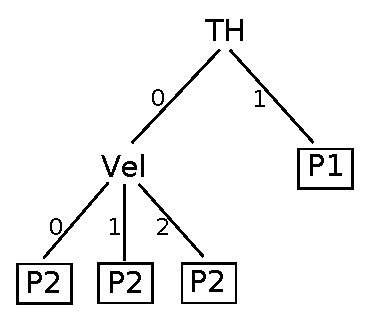
\includegraphics[width=\textwidth]{./EPS/THBaum.eps}
\end{minipage}

\end{frame}

\cleardoublepage

%%%%%%%%%%%%%%%%%%%%%%%%%%%%%%%%%%%%%%%%%%%%%%%%%%%%%%%%%%%%
%%%%%%%%%%%%%%%%%%%%%%%%%%%%%%%%%%%%%%%%%%%%%%%%%%%%%%%%%%%%
%%%%%%%%%%%%%%%%%%%%%%%%%%%%%%%%%%%%%%%%%%%%%%%%%%%%%%%%%%%%
\section{Discrete Functions in \texttt{dune-pdelab}}
%%%%%%%%%%%%%%%%%%%%%%%%%%%%%%%%%%%%%%%%%%%%%%%%%%%%%%%%%%%%
%%%%%%%%%%%%%%%%%%%%%%%%%%%%%%%%%%%%%%%%%%%%%%%%%%%%%%%%%%%%
%%%%%%%%%%%%%%%%%%%%%%%%%%%%%%%%%%%%%%%%%%%%%%%%%%%%%%%%%%%%

\subsection{Local Finite Element Space}

A global finite element space is built up from a collection of local
finite element spaces for each element.

\begin{frame}
\frametitle<presentation>{Local Finite Element Space}
A local finite element space (compare \cite{Ciarlet}) 
is represented by \lstinline{Dune::LocalFiniteElementInterface}
and consists of the following:
\begin{itemize}
\item The type of reference element, given by \lstinline{Dune::GeometryType}.
\item The local basis functions
$\hat\Phi = \{\hat\phi_i : \mathbb{D}^n \to \mathbb{K}^m \,|\, 0\leq i < k\}$
and their gradients in a class derived from \lstinline{Dune::C1LocalBasisInterface}.
\item Information that allows to construct the local to global map $g:
(e,i) \mapsto j$ in a class derived
from \lstinline{Dune::LocalCoefficientsInterface}. 
\item A method that allows to compute coefficients $z_i$ such that
\begin{equation*}
\sum_{0\leq i < k} z_i \hat\phi_i = \hat{u} \qquad \hat{u}\in\text{span}\hat\Phi 
\end{equation*} 
in a class derived
from \lstinline{Dune::LocalInterpolationInterface}. For
$\hat{u}\not\in\text{span}\hat\Phi$ the method provides a projection.
\item The dune module \lstinline{dune-localfunctions} provides a
collection of local finite element spaces.
\end{itemize}
\end{frame}

\begin{frame}[fragile]
\frametitle<presentation>{Function Traits}
The local basis is required to contain a class \lstinline{Traits} that
gives the types for
$\mathbb{D}, \mathbb{D}^n, \mathbb{K}, \mathbb{K}^m$, the numbers $n$,
$m$ and a type for the Jacobian:
\begin{lstlisting}[basicstyle=\ttfamily\scriptsize,numbers=left, 
numberstyle=\tiny, numbersep=5pt]
template<class DF, int n, class D, class RF, int m, class R>
struct C0LocalBasisTraits 
{
  typedef DF DomainFieldType; typedef D DomainType;
  typedef RF RangeFieldType;  typedef R RangeType;
  enum { dimDomain=n }; enum { dimRange=m }; enum { diffOrder=0 };
};
\end{lstlisting}
\begin{lstlisting}[basicstyle=\ttfamily\scriptsize,numbers=left, 
numberstyle=\tiny, numbersep=5pt]
template<class DF, int n, class D, class RF, int m, class R, class J>
struct C1LocalBasisTraits : public C0LocalBasisTraits<DF,n,D,RF,m,R> 
{
  typedef J JacobianType; enum { diffOrder=1 };
};
\end{lstlisting}

Note: Basis functions may be vector-valued.

Later on, other classes representing functions will use the same
traits classes.
\end{frame}

\begin{frame}
\frametitle<presentation>{$Q_1$ Local Basis}
We now consider the bilinear elements $Q_1$ as an example.

The basis functions are given by
\begin{align*}
\hat\phi_2(\hat{x}) &= (1-\hat{x}_0)\hat{x}_1, &
\hat\phi_3(\hat{x}) &= \hat{x}_0\hat{x}_1, \\
\hat\phi_0(\hat{x}) &= (1-\hat{x}_0)(1-\hat{x}_1), &
\hat\phi_1(\hat{x}) &= \hat{x}_0(1-\hat{x}_1).
\end{align*}


\begin{columns}
\begin{column}{0.65\textwidth}
The numbering of the basis functions corresponds to the reference
quadrilateral.
\end{column}
\mode<presentation>{
\begin{column}{0.3\textwidth}
\includegraphics[width=\textwidth]{./EPS/quadrilateral.eps}
\end{column}}
\end{columns}

\mode<article>{
\begin{figure}
\begin{center}
\includegraphics[width=0.5\textwidth]{./EPS/quadrilateral.eps}
\end{center}
\caption{DUNE reference quadrilateral.}
\end{figure}}
\end{frame}

\begin{frame}[fragile]
\frametitle<presentation>{$Q_1$ Local Basis Implementation}
The following listing gives an implementation of the local basis
functions. 

The base class \lstinline{Dune::C1LocalBasisInterface} provides
provides a Barton-Nackman style interface base class for
differentiable basis functions.

This interface will be extended to provide also higher derivatives.

There is also an interface \lstinline{Dune::C0LocalBasisInterface}
when no derivatives are provided.

Evaluation always provides the values of \textit{all} basis functions
or gradients at \textit{one} point. 

Implementations typically use \lstinline{Dune::FieldVector<T,n>} to
represent short vectors.

\lstinline{JacobianType} is \lstinline{Dune::FieldVector<Dune::FieldVector<R,2>,1>}.

In the jacobian evaluation in lines \ref{q1b:grad0} to \ref{q1b:grad3}
we have
\begin{equation*}
\text{\lstinline{out[i][j][k]}}
= \partial_{\hat{x}_k} \left(\hat\phi_i\right)_j (\hat{x}) . 
\end{equation*}
\end{frame}


\begin{frame}<presentation>[fragile,allowframebreaks,allowdisplaybreaks]
\frametitle<presentation>{$Q_1$ Local Basis Listing}
\framesubtitle<presentation>{File \texttt{examples/q1localbasis.hh}}
\lstinputlisting[basicstyle=\ttfamily\scriptsize,numbers=left, 
numberstyle=\tiny, numbersep=5pt]{../../examples/q1localbasis.hh}
\end{frame}
\mode<article>{
\begin{Lst}[File examples/q1localbasis.hh] \mbox
\nopagebreak
\lstinputlisting[basicstyle=\ttfamily\scriptsize,numbers=left, 
numberstyle=\tiny, numbersep=5pt]{../../examples/q1localbasis.hh}
\end{Lst}}


\begin{frame}
\frametitle<presentation>{$Q_1$ Local Coefficients}
In order to provide (different forms of) continuity of \textit{global} basis
functions local indices in \textit{adjacent} elements need to be \textit{identified}.

This is done via (sub-)entities of a given codim 0 entity.

\textit{On the reference element} each local index $0\leq i < k$ is
mapped to
\begin{itemize}
\item a subentity given by a number and a codimension.
\item an offset with in that entity if several indices are mapped to
the same subentity (offset is zero if only one local index is mapped
to the subentity). 
\end{itemize} 

From this information a local-to-global map $g$ can be
constructed \textit{generically}. 

Class \lstinline{Dune::LocalKey} collects subentity and offset information.

For the $Q_1$ element the code is given by the following listing.
\end{frame}

\begin{frame}<presentation>[fragile,allowframebreaks,allowdisplaybreaks]
\frametitle<presentation>{$Q_1$ Local Coefficients Listing}
\framesubtitle<presentation>{File \texttt{examples/q1localcoefficients.hh}}
\lstinputlisting[basicstyle=\ttfamily\scriptsize,numbers=left, 
numberstyle=\tiny, numbersep=5pt]{../../examples/q1localcoefficients.hh}
\end{frame}
\mode<article>{
\begin{Lst}[File examples/q1localcoefficients.hh] \mbox
\nopagebreak
\lstinputlisting[basicstyle=\ttfamily\scriptsize,numbers=left, 
numberstyle=\tiny, numbersep=5pt]{../../examples/q1localcoefficients.hh}
\end{Lst}}


\begin{frame}
\frametitle<presentation>{$Q_1$ Local Interpolation}
Local interpolation takes a function $\hat{u}(\hat{x})$ \textit{on the
reference element} and provides a projection onto the space spanned by
the local basis.

For Lagrange basis functions this is point-wise evaluation.

For other basis functions this might involve the solution of a local
system (e.g. $L_2$-projection).

The local interpolation interface is provided by
\lstinline{Dune::LocalInterpolationInterface}.
\end{frame}


\begin{frame}<presentation>[fragile,allowframebreaks,allowdisplaybreaks]
\frametitle<presentation>{$Q_1$ Local Interpolation Listing}
\framesubtitle<presentation>{File \texttt{examples/q1localinterpolation.hh}}
\lstinputlisting[basicstyle=\ttfamily\scriptsize,numbers=left, 
numberstyle=\tiny, numbersep=5pt]{../../examples/q1localinterpolation.hh}
\end{frame}
\mode<article>{
\begin{Lst}[File examples/q1localinterpolation.hh] \mbox
\nopagebreak
\lstinputlisting[basicstyle=\ttfamily\scriptsize,numbers=left, 
numberstyle=\tiny, numbersep=5pt]{../../examples/q1localinterpolation.hh}
\end{Lst}}

\begin{frame}
\frametitle<presentation>{$Q_1$ Local Interpolation Finite Element}
Finally, we need to collect local basis, local coefficients and local
interpolation in a local finite element.

Local finite element also provides the reference element.

The interface is given
in \lstinline{Dune::LocalFiniteElementInterface}.

Currently (March 2009), \lstinline{dune-localfunctions} implements the
following elements:
\begin{itemize}
\item Piecewise constant elements $P_0$ for any reference element in any
dimension. 
\item Piecewise linear Lagrange elements $P_1$ in $1, 2, 3d$.
\item Piecewise multi-linear Lagrange elements $Q_1$ in $1, 2, 3d$.
\item $P_k$ on triangles.
\item $Q_2$ on quadrilaterals.
\item Lowest order Raviart-Thomas elements on triangles. 
\end{itemize}
\end{frame}

\begin{frame}<presentation>[fragile,allowframebreaks,allowdisplaybreaks]
\frametitle<presentation>{$Q_1$ Local Finite Element Listing}
\framesubtitle<presentation>{File \texttt{examples/q1localfiniteelement.hh}}
\lstinputlisting[basicstyle=\ttfamily\scriptsize,numbers=left, 
numberstyle=\tiny, numbersep=5pt]{../../examples/q1localfiniteelement.hh}
\end{frame}
\mode<article>{
\begin{Lst}[File examples/q1localfiniteelement.hh] \mbox
\nopagebreak
\lstinputlisting[basicstyle=\ttfamily\scriptsize,numbers=left, 
numberstyle=\tiny, numbersep=5pt]{../../examples/q1localfiniteelement.hh}
\end{Lst}}


\subsection{Unconstrained Global Finite Element Space}

\begin{frame}
\frametitle<presentation>{Finite Element Map}
A global finite element space is made up from a collection of local
finite element spaces. 

So we need a map that delivers for each element (codim 0 entity) $e\in E_h^0$ a
local finite element.

But there is only one \textit{type} for all the local finite elements
which then has to be polymorphic.

For multi-element type meshes and $hp$-refinement this map may be
rather complicated.

In our implementation of $P_k$ elements for $k>2$ we use the map to
match the degrees of freedom on common edges and faces.

For the special case where we have \textit{the same} local finite
element for \textit{all} the elements there is a default implementation that is
used in the following listing.
\end{frame}

\begin{frame}<presentation>[fragile,allowframebreaks,allowdisplaybreaks]
\frametitle<presentation>{$Q_1$ Local Finite Element Map Listing}
\framesubtitle<presentation>{File \texttt{examples/q1localfiniteelementmap.hh}}
\lstinputlisting[basicstyle=\ttfamily\scriptsize,numbers=left, 
numberstyle=\tiny, numbersep=5pt]{../../examples/q1localfiniteelementmap.hh}
\end{frame}
\mode<article>{
\begin{Lst}[File examples/q1localfiniteelementmap.hh] \mbox
\nopagebreak
\lstinputlisting[basicstyle=\ttfamily\scriptsize,numbers=left, 
numberstyle=\tiny, numbersep=5pt]{../../examples/q1localfiniteelementmap.hh}
\end{Lst}}


\begin{frame}
\frametitle<presentation>{$Q_1$ Grid Function Space}
Now use $Q_1$ local finite element to build
a global finite element space.

The main class is \lstinline{GridFunctionSpace} which 
builds up the local to global map $g$ and provides information about
the local finite elements.

An element of the function space is represented by a coefficient
vector that is
encapsulated in a seperate type, see definition \lstinline{X}.

The type \lstinline{X} is derived from \lstinline{std::vector<R>} here
but his will be changed later.

The remaining lines construct a function object that can be evaluated
in local coordinates on the reference element.

\lstinline{Dune::SubsamplingVTKWriter} allows the output of
nonconforming and higher order functions.
\end{frame}

\begin{frame}<presentation>[fragile,allowframebreaks,allowdisplaybreaks]
\frametitle<presentation>{$Q_1$ Grid Function Space Listing}
\framesubtitle<presentation>{File \texttt{examples/q1gridfunctionspace.hh}}
\lstinputlisting[basicstyle=\ttfamily\scriptsize,numbers=left, 
numberstyle=\tiny, numbersep=5pt]{../../examples/q1gridfunctionspace.hh}
\end{frame}
\mode<article>{
\begin{Lst}[File examples/q1gridfunctionspace.hh] \mbox
\nopagebreak
\lstinputlisting[basicstyle=\ttfamily\scriptsize,numbers=left, 
numberstyle=\tiny, numbersep=5pt]{../../examples/q1gridfunctionspace.hh}
\end{Lst}}

\begin{frame}
\frametitle<presentation>{$Q_1$ Grid Function Space Main Program}
Finally, in the main program a \lstinline{Dune::Grid} is instantiated
and the generic function is called.

We show only one main program here for illustration. In the other
examples below the main programs will not be listed.
\end{frame}

\begin{frame}<presentation>[fragile,allowframebreaks,allowdisplaybreaks]
\frametitle<presentation>{$Q_1$ GFS Main Program Listing}
\framesubtitle<presentation>{File \texttt{examples/q1gridfunctionspacemain.cc}}
\lstinputlisting[basicstyle=\ttfamily\scriptsize,numbers=left, 
numberstyle=\tiny, numbersep=5pt]{../../examples/q1gridfunctionspacemain.cc}
\end{frame}
\mode<article>{
\begin{Lst}[File examples/q1gridfunctionspacemain.cc] \mbox
\nopagebreak
\lstinputlisting[basicstyle=\ttfamily\scriptsize,numbers=left, 
numberstyle=\tiny, numbersep=5pt]{../../examples/q1gridfunctionspacemain.cc}
\end{Lst}}


\begin{frame}<presentation>
\frametitle<presentation>{$Q_1$ Global Basis Function Visualization}
\begin{center}
\includegraphics[width=0.65\textwidth]{./EPS/q1.eps}
\end{center}
\end{frame}

Figure \ref{fig:Q1GlobalBasisFunction} shows the result visualized
with ParaView.

\mode<article>{
\begin{figure}
\begin{center}
\includegraphics[width=0.5\textwidth]{./EPS/q1.eps}
\end{center}
\caption{$Q_1$ global basis function visualized with ParaView.}
\label{fig:Q1GlobalBasisFunction}
\end{figure}
}

\subsection{Interpolation from Analytic Function}

\mode<article>{
\begin{figure}
\begin{center}
\includegraphics[width=0.5\textwidth]{./EPS/q1interpolate.eps}
\end{center}
\caption{Interpolation of $\exp(-3\|x-c\|^2)$ with $Q_1$ elements.}
\label{fig:Q1Interpolation}
\end{figure}
}

\begin{frame}
\frametitle<presentation>{Functions}
Often one wants to prescribe functions for initial or boundary
conditions.

PDELab offers several classes to represent functions:
\begin{itemize}
\item \lstinline{Dune::PDELab::FunctionInterface} is the interface for general
functions $$u : \mathbb{D}^n \to \mathbb{K}^m, \qquad x \mapsto y.$$ 
\item \lstinline{Dune::PDELab::GridFunctionInterface} is the interface
for functions defined on a grid:
$$u : E_h^0 \times \mathbb{D}^n \to \mathbb{K}^m, \qquad
(e,\hat{x}) \mapsto y.$$
$\hat{x}$ is on the \textit{reference element}.
\item \lstinline{Dune::PDELab::BoundaryGridFunctionInterface} is the
interface for \textit{grid functions} living on the boundary:
$$u : (E_h^1\cap\partial\Omega) \times \mathbb{D}^{n'} \to \mathbb{K}^m, \qquad
(f,\hat{x}) \mapsto y.$$
\item Functions offer the same \lstinline{Traits} as the local basis.
\end{itemize}
\end{frame}


\begin{frame}
\frametitle<presentation>{Useful Adapters and Base Classes}
There are various useful adapters and base classes:

\lstinline{Dune::PDELab::DiscreteGridFunction}: Takes a grid
function space and a coefficient vector and makes a grid function out
of it.

\lstinline{Dune::PDELab::VTKGridFunctionAdapter}: Takes a grid
function and makes a VTK function out of it (this is the input
for \lstinline{VTKWriter}). These two classes have been used already above.

\lstinline{Dune::PDELab::AnalyticGridFunctionBase}: Implements
grid function interface from global function by deriving from it.
This class will be used shortly.

\end{frame}

\begin{frame}
\frametitle<presentation>{Less Useful Adapters}
\lstinline{Dune::PDELab::FunctionToGridFunctionAdapter}: Takes a global
function and makes a grid function out of it.

\lstinline{Dune::PDELab::GlobalFunctionToLocalFunctionAdapter}:
Takes a global function and an element and provides evaluation
w.r.t.~reference element.

\lstinline{Dune::PDELab::GridFunctionToLocalFunctionAdapter}:
Takes grid function and element, acts as function on the
reference element.

\lstinline{Dune::PDELab::SelectComponentAdapter}. Takas
vector-valued function and component number and provides a scalar function.

\lstinline{D...::BoundaryGridFunctionSelectComponentAdapter}:
Same for boundary grid functions.

\lstinline{Dune::PDELab::PiolaBackwardAdapter}: Takes global
vector-valued function, makes grid function tranformed back to
reference element.

For more details see \lstinline{dune/pdelab/common/function.hh}.
\end{frame}

\begin{frame}<presentation>[fragile,allowframebreaks,allowdisplaybreaks]
\frametitle<presentation>{\texttt{AnalyticGridFunctionBase} Example Listing}
\framesubtitle<presentation>{File \texttt{examples/analyticfunction.hh}}
\lstinputlisting[basicstyle=\ttfamily\scriptsize,numbers=left, 
numberstyle=\tiny, numbersep=5pt]{../../examples/analyticfunction.hh}
\end{frame}
\mode<article>{
\begin{Lst}[File examples/analyticfunction.hh] \mbox
\nopagebreak
\lstinputlisting[basicstyle=\ttfamily\scriptsize,numbers=left, 
numberstyle=\tiny, numbersep=5pt]{../../examples/analyticfunction.hh}
\end{Lst}}

\begin{frame}
\frametitle<presentation>{Generic Interpolation}
Interpolation of a finite element function from a given function is
now generic.
\end{frame}


\begin{frame}<presentation>[fragile,allowframebreaks,allowdisplaybreaks]
\frametitle<presentation>{Generic Interpolation Listing}
\framesubtitle<presentation>{File \texttt{examples/q1interpolate.hh}}
\lstinputlisting[basicstyle=\ttfamily\scriptsize,numbers=left, 
numberstyle=\tiny, numbersep=5pt]{../../examples/q1interpolate.hh}
\end{frame}
\mode<article>{
\begin{Lst}[File examples/q1interpolate.hh] \mbox
\nopagebreak
\lstinputlisting[basicstyle=\ttfamily\scriptsize,numbers=left, 
numberstyle=\tiny, numbersep=5pt]{../../examples/q1interpolate.hh}
\end{Lst}}

\begin{frame}<presentation>
\frametitle<presentation>{Visualization of the Result}
\begin{center}
\includegraphics[width=0.65\textwidth]{./EPS/q1interpolate.eps}
\end{center}
\end{frame}



\subsection{Interpolation Error}

\begin{frame}
\frametitle<presentation>{Interpolation Error Example}
Now, we do a little example that shows how one can work with global
finite element functions.

For a given function $u$ and its interpolant $u_h\in
U_h(\mathbb{T}_h)$ we want to compute the $L_2$ interpolation error 
\begin{equation*}
\begin{split}
\|&u-u_h\|_{L_2(\Omega)} = \int_\Omega (u-u_h)^2\, dx 
= \sum_{e\in E_h^0} \int_{\Omega_e} (u-u_h)^2\, dx \\
&= \sum_{e\in E_h^0} \int_{\hat{\Omega}_e} \left(u(\mu_e(\hat{x})) -
u_h(\mu_e(\hat{x})) \right)^2 \text{det} \nabla\mu_e(\hat{x}) \,
d\hat{x}\\
&= \sum_{e\in E_h^0} \sum_{j=0}^{q(e)-1} w_{e,j} \left( u(\mu_e(\hat{x}_{e,j})) -
u_h(\mu_e(\hat{x}_{e,j})) \right)^2 \text{det} \nabla\mu_e(\hat{x}_{e,j}) \,
d\hat{x} \text{ $+$ error}\\
&= \sum_{e\in E_h^0} \sum_{j=0}^{q(e)-1} w_{e,j} \left(u(\mu_e(\hat{x}_{e,j})) -
\sum_{i=0}^{k(e)-1}(\mathbf{u})_{g(e,i)} \hat\phi_{e,i}(\hat{x}_{e,j}) \right)^2  
\text{det} \nabla\mu_e(\hat{x}_{e,j}) \,  
d\hat{x} \text{ $+$ error} .
\end{split}
\end{equation*}
\end{frame}

\begin{frame}
\frametitle<presentation>{Interpolation Error Example}
In the following code example the
function \lstinline{l2interpolationerror} is parametrized by
\begin{itemize}
\item \lstinline{U}: Type for a function. 
\item \lstinline{GFS}: Type for a grid function space.
\item \lstinline{X}: Type for a coefficient vector.
\end{itemize}
The local function space
\lstinline{GFS::LocalFunctionSpace} in line \ref{l2int:lfs} is a type 
exported by a grid function space which
\begin{itemize}
\item is bound to an element $e$ later in line \ref{l2int:bind},
\item provides the local finite element for that element $e$ ,
\item provides the local to global map $g(e,\cdot)$ for that element,
\item can read, write and add degrees of freedom of element $e$.
\end{itemize}
\lstinline{Dune::QuadratureRule} in line \ref{l2int:quad} provides
quadrature rules for many element types, dimensions and orders.
\end{frame}

\begin{frame}<presentation>[fragile,allowframebreaks,allowdisplaybreaks]
\frametitle<presentation>{Interpolation Error Listing}
\framesubtitle<presentation>{File \texttt{examples/l2interpolationerror.hh}}
\lstinputlisting[basicstyle=\ttfamily\scriptsize,numbers=left, 
numberstyle=\tiny, numbersep=5pt]{../../examples/l2interpolationerror.hh}
\end{frame}
\mode<article>{
\begin{Lst}[File examples/l2interpolationerror.hh] \mbox
\nopagebreak
\lstinputlisting[basicstyle=\ttfamily\scriptsize,numbers=left, 
numberstyle=\tiny, numbersep=5pt]{../../examples/l2interpolationerror.hh}
\end{Lst}}

Next comes the driver that uses the generic $L_2$ interpolation error
function.

\begin{frame}<presentation>[fragile,allowframebreaks,allowdisplaybreaks]
\frametitle<presentation>{Interpolation Error Driver Listing}
\framesubtitle<presentation>{File \texttt{examples/q1interpolationerror.hh}}
\lstinputlisting[basicstyle=\ttfamily\scriptsize,numbers=left, 
numberstyle=\tiny, numbersep=5pt]{../../examples/q1interpolationerror.hh}
\end{frame}
\mode<article>{
\begin{Lst}[File examples/q1interpolationerror.hh] \mbox
\nopagebreak
\lstinputlisting[basicstyle=\ttfamily\scriptsize,numbers=left, 
numberstyle=\tiny, numbersep=5pt]{../../examples/q1interpolationerror.hh}
\end{Lst}}

\begin{frame}[fragile]
\frametitle<presentation>{$Q_1$ Interpolation Error}
Evaluating the interpolaton error for our $Q_1$ basis for different
levels of refinement produces the following result:
\begin{lstlisting}[basicstyle=\ttfamily\scriptsize]
interpolation error:        1 elements 4.63081768e-01
interpolation error:        4 elements 1.02612039e-01
interpolation error:       16 elements 3.03000305e-02
interpolation error:       64 elements 7.77518775e-03
interpolation error:      256 elements 1.95618596e-03
interpolation error:     1024 elements 4.89819655e-04
interpolation error:     4096 elements 1.22503221e-04
interpolation error:    16384 elements 3.06288243e-05
interpolation error:    65536 elements 7.65739477e-06
interpolation error:   262144 elements 1.91436048e-06
interpolation error:  1048576 elements 4.78590858e-07
\end{lstlisting}
Obviously, we get second order approximation.
\end{frame}

\begin{frame}
\frametitle<presentation>{Modification for $Q_2$}
Now it is very easy to compute the interpolation error for other
function spaces.

Just replace \lstinline{Q1LocalFiniteElementMap}
with \lstinline{Dune::PDELab::Q22DLocalFiniteElementMap} in
lines \ref{l2int:q2} and \ref{l2int:q22}!
\end{frame}

\begin{frame}<presentation>[fragile,allowframebreaks,allowdisplaybreaks]
\frametitle<presentation>{$Q_2$ Interpolation Error Driver Listing}
\framesubtitle<presentation>{File \texttt{examples/q2interpolationerror.hh}}
\lstinputlisting[basicstyle=\ttfamily\scriptsize,numbers=left, 
numberstyle=\tiny, numbersep=5pt]{../../examples/q2interpolationerror.hh}
\end{frame}
\mode<article>{
\begin{Lst}[File examples/q2interpolationerror.hh] \mbox
\nopagebreak
\lstinputlisting[basicstyle=\ttfamily\scriptsize,numbers=left, 
numberstyle=\tiny, numbersep=5pt]{../../examples/q2interpolationerror.hh}
\end{Lst}}

\begin{frame}[fragile]
\frametitle<presentation>{$Q_2$ Interpolation Error}
And we see third order approximation:
\begin{lstlisting}[basicstyle=\ttfamily\scriptsize]
interpolation error:        1 elements 4.65290291e-02
interpolation error:        4 elements 1.20509875e-02
interpolation error:       16 elements 1.36558258e-03
interpolation error:       64 elements 1.71127393e-04
interpolation error:      256 elements 2.14102072e-05
interpolation error:     1024 elements 2.67692161e-06
interpolation error:     4096 elements 3.34635709e-07
interpolation error:    16384 elements 4.18301070e-08
interpolation error:    65536 elements 5.22878350e-09
interpolation error:   262144 elements 6.53598587e-10
interpolation error:  1048576 elements 8.16998215e-11
\end{lstlisting}
\end{frame}

\subsection{Constrained Global Finite Element Space}

We now show how constraints can be added to a grid function space.

\begin{frame}
\frametitle<presentation>{Adding Constraints to a Grid Function Space}
Constraints are a property of a grid function space.

In addition to the local finite elements we have to
parametrize \lstinline{Dune::PDELab::GridFunctionSpace} with a type
that can provide the sparse transformation matrix
$\mathbf{T}_{\tilde{U}_h,\bar{U}_h}$ from \eqref{Eq:StructureTransformation}. 

Information should be provided only locally. One
column of $\mathbf{T}_{\tilde{U}_h,\bar{U}_h}$ may only involve
degrees of freedom of two (intersecting) elements.

A constraints class provides rows of
$\mathbf{T}^T_{\tilde{U}_h,\bar{U}_h}$ and may have methods
\begin{itemize}
\item \lstinline{volume}: Constrain degrees of freedom associated with
volume (useful in parallelization).
\item \lstinline{skeleton}: Constrain degrees of freedom associated
with interior intersections (useful for hanging nodes).
\item \lstinline{boundary}: Constrain degrees of freedom on boundary
intersections (for boundary conditions).
\end{itemize}
Flags \lstinline{do...} control which methods must be provided.
\end{frame}

\begin{frame}<presentation>[fragile,allowframebreaks,allowdisplaybreaks]
\frametitle<presentation>{Constraints Assembler Listing}
\framesubtitle<presentation>{File \texttt{examples/q1constraints.hh}}
\lstinputlisting[basicstyle=\ttfamily\scriptsize,numbers=left, 
numberstyle=\tiny, numbersep=5pt]{../../examples/q1constraints.hh}
\end{frame}
\mode<article>{
\begin{Lst}[File examples/q1constraints.hh] \mbox
\nopagebreak
\lstinputlisting[basicstyle=\ttfamily\scriptsize,numbers=left, 
numberstyle=\tiny, numbersep=5pt]{../../examples/q1constraints.hh}
\end{Lst}}

\begin{frame}
\frametitle<presentation>{A Boundary Condition Function}
To use assembling of constraints 
we define a boundary grid function that gives the \textit{boundary
condition type} for a point on the boundary.

Note that \lstinline{RangeFieldType} is set to \lstinline{int} in
line \ref{bct:int}.
\end{frame}

\begin{frame}<presentation>[fragile,allowframebreaks,allowdisplaybreaks]
\frametitle<presentation>{Boundary Condition Type Function Listing}
\framesubtitle<presentation>{File \texttt{examples/boundaryconditiontypefunction.hh}}
\lstinputlisting[basicstyle=\ttfamily\scriptsize,numbers=left, 
numberstyle=\tiny, numbersep=5pt]{../../examples/boundaryconditiontypefunction.hh}
\end{frame}
\mode<article>{
\begin{Lst}[File examples/boundaryconditiontypefunction.hh] \mbox
\nopagebreak
\lstinputlisting[basicstyle=\ttfamily\scriptsize,numbers=left, 
numberstyle=\tiny, numbersep=5pt]{../../examples/boundaryconditiontypefunction.hh}
\end{Lst}}

\begin{frame}
\frametitle<presentation>{Interpolation with Constraints}
In the following listing we redo the interpolation example 
with a constrained finite element space.

In line \ref{cint:newparameter} the grid function space is
parametrized with the constraints class.

In line \ref{cint:container} the grid function space exports a type to
hold the transformation matrix
$\mathbf{T}^T_{\tilde{U}_h,\bar{U}_h}$. 

In line \ref{cint:bctfunction} the function giving the boundary
condition type is instantiated.

Finally, in line \ref{cint:constraints} the constraints are assembled
and stored.

Function \lstinline{Dune::PDELab::set_nonconstrained_dofs} in
line \ref{cint:setconstraints} allows to set all nonconstrained
degrees of freedom to a given value.

Function \lstinline{Dune::PDELab::set_constrained_dofs} does the same
for the constrained degrees of freedom.
\end{frame}


\begin{frame}<presentation>[fragile,allowframebreaks,allowdisplaybreaks]
\frametitle<presentation>{Constrained Interpolation Listing}
\framesubtitle<presentation>{File \texttt{examples/q1constrainedinterpolate.hh}}
\lstinputlisting[basicstyle=\ttfamily\scriptsize,numbers=left, 
numberstyle=\tiny, numbersep=5pt]{../../examples/q1constrainedinterpolate.hh}
\end{frame}
\mode<article>{
\begin{Lst}[File examples/q1constrainedinterpolate.hh] \mbox
\nopagebreak
\lstinputlisting[basicstyle=\ttfamily\scriptsize,numbers=left, 
numberstyle=\tiny, numbersep=5pt]{../../examples/q1constrainedinterpolate.hh}
\end{Lst}}

\begin{frame}<presentation>
\frametitle<presentation>{Visualization of Affine Shift Function}
\begin{center}
\includegraphics[width=0.65\textwidth]{./EPS/q1constrainedinterpolate.eps}
\end{center}
\end{frame}

Figure \ref{fig:Q1ConstrainedInterpolation} shows the result obtained
after setting the nonconstrained degrees of freedom to zero.


\mode<article>{
\begin{figure}
\begin{center}
\includegraphics[width=0.5\textwidth]{./EPS/q1constrainedinterpolate.eps}
\end{center}
\caption{Interpolation of $\exp(-3\|x-c\|^2)$ with $Q_1$ elements with
subsequent modification of nonconstrained degrees of freedom.}
\label{fig:Q1ConstrainedInterpolation}
\end{figure}
}

\subsection{Composite Finite Element Spaces}

\mode<article>{
\begin{figure}
\begin{center}
\includegraphics[width=0.5\textwidth]{./EPS/thinterpolate.eps}
\end{center}
\caption{Visualization of velocity field and pressure in the
Taylor-Hood example.}
\label{fig:THInterpolation}
\end{figure}
}

\begin{frame}
\frametitle<presentation>{Composition of Finite Element Spaces}
For systems of PDEs we need product function spaces.

This can be achieved now in a completely generic way:
\begin{itemize}
\item \lstinline{Dune::PDELab::PowerGridFunctionSpace<GFS,k,M>} builds a
new grid function space that is \lstinline{k}-times the product of \lstinline{GFS}.
\item \lstinline{D...::CompositeGridFunctionSpace<M,GFS0,...,GFS8>}
builds a new grid function space out of up to 9 existing grid function
spaces. 
\item \lstinline{M} controls construction of local to global map.
\end{itemize}

This can be applied recursively leading to a type tree.

The local function space reflects this type tree.

\lstinline{Dune::PDELab::GridFunctionSubSpace} allows the selection of
subspaces.

Functions can be composed in a similar way.
\end{frame}

\begin{frame}
\frametitle<presentation>{Taylor-Hood Example}
We now do the Taylor-Hood function space as an example.

As before, we construct the function space and interpolate a finite
element function from a given analytic function.

Let us start by defining a vector-valued analytic function for the
velocity field.  
\end{frame}

\begin{frame}<presentation>[fragile,allowframebreaks,allowdisplaybreaks]
\frametitle<presentation>{Analytic Velocity Field Listing}
\framesubtitle<presentation>{File \texttt{examples/thvelocity.hh}}
\lstinputlisting[basicstyle=\ttfamily\scriptsize,numbers=left, 
numberstyle=\tiny, numbersep=5pt]{../../examples/thvelocity.hh}
\end{frame}
\mode<article>{
\begin{Lst}[File examples/thvelocity.hh] \mbox
\nopagebreak
\lstinputlisting[basicstyle=\ttfamily\scriptsize,numbers=left, 
numberstyle=\tiny, numbersep=5pt]{../../examples/thvelocity.hh}
\end{Lst}}

Now the Taylor-Hood interpolation example.

\begin{frame}<presentation>[fragile,allowframebreaks,allowdisplaybreaks]
\frametitle<presentation>{Taylor Hood Example Listing}
\framesubtitle<presentation>{File \texttt{examples/thinterpolate.hh}}
\lstinputlisting[basicstyle=\ttfamily\scriptsize,numbers=left, 
numberstyle=\tiny, numbersep=5pt]{../../examples/thinterpolate.hh}
\end{frame}
\mode<article>{
\begin{Lst}[File examples/thinterpolate.hh] \mbox
\nopagebreak
\lstinputlisting[basicstyle=\ttfamily\scriptsize,numbers=left, 
numberstyle=\tiny, numbersep=5pt]{../../examples/thinterpolate.hh}
\end{Lst}}

\begin{frame}<presentation>
\frametitle<presentation>{Visualization of Taylor-Hood Function}
\begin{center}
\includegraphics[width=0.5\textwidth]{./EPS/thinterpolate.eps}
\end{center}
\end{frame}

Figure \ref{fig:THInterpolation} visualizes the result of this
example.

\subsection{Summary}

\begin{frame}
\frametitle<presentation>{Function Space Summary}
In order to incorporate a function space in PDELab do the following: 
\begin{itemize}
\item Hope that somebody already included the local basis
in \texttt{dune-localfunctions} and provided the finite element map
in \texttt{dune-pdelab}. 
\item If not, you have to
\begin{itemize}
\item Make a local basis.
\item Make local coefficients.
\item Make a local interpolation.
\item Make a finite element.
\item Make a finite element map.
\end{itemize}
\item Write a constraints assembler if required.
\item Set up the function space via \texttt{GridFunctionSpace}
\end{itemize}
\end{frame}

\cleardoublepage

%%%%%%%%%%%%%%%%%%%%%%%%%%%%%%%%%%%%%%%%%%%%%%%%%%%%%%%%%%%%
%%%%%%%%%%%%%%%%%%%%%%%%%%%%%%%%%%%%%%%%%%%%%%%%%%%%%%%%%%%%
%%%%%%%%%%%%%%%%%%%%%%%%%%%%%%%%%%%%%%%%%%%%%%%%%%%%%%%%%%%%
\section{Algebraic Formulation}
%%%%%%%%%%%%%%%%%%%%%%%%%%%%%%%%%%%%%%%%%%%%%%%%%%%%%%%%%%%%
%%%%%%%%%%%%%%%%%%%%%%%%%%%%%%%%%%%%%%%%%%%%%%%%%%%%%%%%%%%%
%%%%%%%%%%%%%%%%%%%%%%%%%%%%%%%%%%%%%%%%%%%%%%%%%%%%%%%%%%%%

\subsection{Solution of the Unconstrained Problem}

\paragraph{Unconstrained Problem in Original Basis}

\begin{frame}
\frametitle<presentation>{Unconstrained Problem in Original Basis}
We recall the unconstrained problem in weighted residual form:
\begin{equation}
u_h\in U_h\ : \qquad r_h(u_h,v) = 0 \qquad \forall
v\in V_h .
\end{equation}

Solving it in the original basis
reduces to the solution of a nonlinear algebraic problem:
\begin{equation}
\begin{split}
\mathbf{u}\in\mathbf{U} : \qquad
& r_h\left(\text{FE}_{\Phi_{U_h}}(\mathbf{u}),\psi_i\right) = 0, \quad
i\in\mathcal{I}_{V_h} \\
\Leftrightarrow \  & \mathcal{R}(\mathbf{u}) = \mathbf{0}
\end{split}
\end{equation}
where we introduced the nonlinear residual map $\mathcal{R} :
\mathbf{U} = \mathbb{K}^{\mathcal{I}_{V_h}} \to \mathbb{K}^{\mathcal{I}_{V_h}}$ which is defined as 
\begin{equation}
\left(
\mathcal{R}(\mathbf{u})\right)_i =
r_h(\text{FE}_{U_h}(\mathbf{u}),\psi_i).
\end{equation}
$\Phi_{V_h} = \{\psi_i\,|\, i\in\mathcal{I}_{V_h}\}$ is the basis of $V_h$.  
\end{frame}

\paragraph{Unconstrained Problem in Transformed Basis}

\begin{frame}
\frametitle<presentation>{Unconstrained Problem in Transformed Basis}
We may also solve the unconstrained problem 
in the transformed basis for trial and test space:
\begin{equation}\label{Eq:TransformedUnconstrainedProblem}
\begin{split}
\mathbf{u}'\in\mathbf{U}' : \qquad 
& r_h\left(\text{FE}_{\Phi'_{U_h}}(\mathbf{u}'),\psi_i'\right) = 0, \quad
i\in\mathcal{I}_{V_h}\\
\Leftrightarrow \  &
r_h\left(\text{FE}_{\Phi_{U_h}}(\mathbf{T}^T_{U_h}\mathbf{u}'),
\sum_{j\in\mathcal{I}_{V_h}}\left(\mathbf{T}_{V_h}\right)_{i,j}\psi_j\right) = 0, \quad
i\in\mathcal{I}_{V_h}\\
\Leftrightarrow \  &
\sum_{j\in\mathcal{I}_{V_h}} \left(\mathbf{T}_{V_h}\right)_{i,j} 
r_h\left(\text{FE}_{\Phi_{U_h}}(\mathbf{T}^T_{U_h}\mathbf{u}'),
\psi_j\right) = 0, \quad
i\in\mathcal{I}_{V_h}\\
\Leftrightarrow \  &
\mathbf{T}_{V_h} \mathcal{R}\left(\mathbf{T}^T_{U_h}\mathbf{u}'\right)
= \mathbf{0} .
\end{split}
\end{equation}
Used linearity of residual form with respect to the second argument.

Requires simple matrix multiplication.
\end{frame}

\paragraph{Newton solver}

Use Newton's method to solve the algebraic problem.

\begin{frame}
\frametitle<presentation>{Newton Solver}
Let a current iterate $\mathbf{u}_k'$ be given. 

We seek an update $\mathbf{z}'_k$ such that $\mathbf{u}'_{k+1} = \mathbf{u}_k'
+ \mathbf{z}'_k$ and linearize:
\begin{equation*}
\mathbf{T}_{V_h}\mathcal{R}\left(\mathbf{T}^T_{U_h}\mathbf{u}'_{k+1}\right) \approx 
\mathbf{T}_{V_h}\mathcal{R}\left(\mathbf{T}^T_{U_h}\mathbf{u}'_{k}\right) +
\mathbf{T}_{V_h}\nabla\mathcal{R}\left(\mathbf{T}^T_{U_h}\mathbf{u}'_{k}\right) 
\mathbf{T}^T_{U_h} \mathbf{z}'_{k} = \mathbf{0} .
\end{equation*}

A linear system for the update is 
\begin{equation}\label{eq:UnconstrainedUpdate}
\mathbf{T}_{V_h}\nabla\mathcal{R}\left(\mathbf{T}^T_{U_h}\mathbf{u}'_{k}\right) 
\mathbf{T}^T_{U_h} \mathbf{z}'_{k} = -
\mathbf{T}_{V_h}\mathcal{R}\left(\mathbf{T}^T_{U_h}\mathbf{u}'_{k}\right) .
\end{equation}

$\nabla\mathcal{R}\left(\mathbf{u}_{k}\right)$ denotes the
Jacobian matrix of the map $\mathcal{R}$. 

Multiplying the update equation with $\mathbf{T}^T_{U_h}$ from the left yields
\begin{equation}\label{eq:OriginalUpdate}
\mathbf{T}^T_{U_h}\mathbf{u}'_{k+1} = \mathbf{T}^T_{U_h}\mathbf{u}_k' +
\mathbf{T}^T_{U_h}\mathbf{z}'_k .
\end{equation}

Setting $\mathbf{u}_{k} := \mathbf{T}^T_{U_h}\mathbf{u}_k'$ allows us
now to write the Newton scheme with respect to the original basis.
\end{frame}


\begin{frame}
\frametitle<presentation>{Newton Solver (Contd.)}
\begin{Alg}[Newton's method for unconstrained problem]
Given the initial guess $\mathbf{u}_{0}$ iterate until convergence
\begin{enumerate}[i)]
\item Compute residual:
  $\mathbf{r}_k=\mathcal{R}\left(\mathbf{u}_{k}\right)$.
\item Transform residual: $\mathbf{r}_k' = \mathbf{T}_{V_h}
  \mathbf{r}_k$.
\item Solve update equation:
  $\mathbf{T}_{V_h}\nabla\mathcal{R}\left(\mathbf{u}_{k}\right)  
\mathbf{T}^T_{U_h} \mathbf{z}'_{k} =  \mathbf{r}_k'$.
\item Transform update: $\mathbf{z}_{k} =
  \mathbf{T}^T_{U_h}\mathbf{z}'_k$.
\item Update: $\mathbf{u}_{k+1} = \mathbf{u}_k
- \mathbf{z}_k$. \hfill$\square$
\end{enumerate}
\end{Alg}

Two applications of the basis transformation, for the
residual and the update, are necessary in steps ii) and iv).

These transformations are cheap due to the structure of the
transformation.

In step (iii) the \textit{transformed}
Jacobian system is required.

\textit{All these transformations are done generically by PDELab}!
\end{frame}

\subsection{Solution of Constrained Problem}

We now turn to the constrained problem.

\paragraph{Reformulation in unconstrained space}

\begin{frame}
\frametitle<presentation>{Reformulation in unconstrained space}
We recall the constrained problem in weighted residual form:
\begin{equation}\label{Eq:ConstrainedProblem}
u_h\in w_h + \tilde{U}_h\ : \qquad r_h(u_h,v) = 0 \quad \forall
v\in \tilde{V}_h .
\end{equation}

This problem can be reformulated in the unconstrained space by adding
a constrained equation:
\begin{Prp}
Let $P_h : U_h \to \tilde{U}_h$ be a projection (i.~e.~$P_h^2 = P_h$)
and assume that the affine shift is such that $P_h w_h = 0$. Then 
\begin{equation}\label{Eq:ConstrainedProblemReformII}
u_h\in U_h\ : \qquad \left\{\begin{array}{ll}
r_h(u_h,v) = 0 \quad \forall v\in \tilde{V}_h\\
(I-P_h)u_h = w_h
\end{array}\right. 
\end{equation}
is equivalent to \eqref{Eq:ConstrainedProblem}.

\mode<article>{
\textit{Proof}. Assume that \eqref{Eq:ConstrainedProblem} holds and
$P_h w_h = 0$. Since $u_h$ solves \eqref{Eq:ConstrainedProblem}
the first equation in \eqref{Eq:ConstrainedProblemReformII} clearly holds.
Moreover, we have $u_h = w_h + \tilde{u}_h$ with $\tilde{u}_h\in
\tilde{U}_h$ which allows us to write $u_h = w_h + P_h v_h$ for some
$v_h\in U_h$. When we can prove that $v_h=u_h$ we obtain the desired
$(I-P_h)u_h = w_h$. We now show that $v_h=u_h$:
Applying $P_h$ to both sides of the identity $u_h = w_h + P_h v_h$ yields
$P_h u_h = P_h w_h + P_h^2 v_h$. Using $P_h w_h = 0$ and $P_h^2 = P_h$
yields $P_h u_h = P_h v_h$. Thus we may identify $v_h$ and $u_h$ as
$v_h$ was arbitrary.\\
Assume now that \eqref{Eq:ConstrainedProblemReformII} holds. The first
equation of \eqref{Eq:ConstrainedProblemReformII} is the same as 
\eqref{Eq:ConstrainedProblem}. From the
second equation we conclude $u_h = w_h + P_h u_h$, i.~e.~ $u_h\in w_h
+ \tilde{U}_h$.} \hfill$\square$
\end{Prp}
\end{frame}

\paragraph{Reformulated Problem in Coefficient Space} 

We now seek to solve problem
\eqref{Eq:ConstrainedProblemReformII} in coefficient space. 

\begin{frame}
\frametitle<presentation>{Reformulated Problem in Coefficient Space}
The projection $P_h$ is taken from the follwing commutative diagram:
\begin{equation*}
\begin{CD}
U_h @>{P_h = \text{FE}_{\Phi'_{U_h}}
\mathbf{R}^T_{\tilde{\mathbf{U}}',\mathbf{U}'}
\mathbf{R}_{\tilde{\mathbf{U}}',\mathbf{U}'} 
\text{FE}_{\Phi'_{U_h}}^{-1}}>> \tilde{U}_h\\
@A{\text{FE}_{\Phi'_{U_h}}}AA @AA{\text{FE}_{\Phi'_{U_h}}
\mathbf{R}^T_{\tilde{\mathbf{U}}'\mathbf{U}'}}A\\
\mathbf{U}' @>{\qquad\mathbf{R}_{\tilde{\mathbf{U}}',\mathbf{U}'}\qquad}>> \tilde{\mathbf{U}}' 
\end{CD}
\end{equation*}

\begin{Prp}
Using this definition of $P_h$ the reformulated constrained
problem \eqref{Eq:ConstrainedProblemReformII} in coefficient space reads
\begin{equation}\label{Eq:ConstrainedProblemInCoefficientSpace}
\mathbf{u}'\in\mathbf{U}' : \qquad \left\{\begin{array}{rcl}
\mathbf{S}_{\tilde{\mathbf{V}}'}
\mathcal{R}\left(\mathbf{T}^T_{U_h}\mathbf{u}'\right)
& = & \mathbf{0}\\
\mathbf{R}_{\bar{\mathbf{U}}',\mathbf{U}'} \mathbf{u}' & = & \mathbf{w}'
\end{array}\right.
\end{equation}
with $\mathbf{S}_{\tilde{\mathbf{V}}'}=\mathbf{R}_{\tilde{\mathbf{V}}',\mathbf{V}'} +
\mathbf{T}_{\tilde{V}_h,\bar{V}_h}\mathbf{R}_{\bar{\mathbf{V}}',\mathbf{V}'}$
and $w_h =
FE_{\Phi_{U_h}'}(\mathbf{R}_{\bar{\mathbf{U}}',\mathbf{U}'}^T\mathbf{w}')$.
\hfill$\square$
\end{Prp}
\end{frame}

The idea in this formulation is that with respect to the transformed
basis the affine shift (for Dirichlet boundary conditions) can be
``encoded'' in the constrained degrees of freedom
$\mathbf{R}_{\bar{\mathbf{U}}',\mathbf{U}'} \mathbf{u}'$. This is
possible because the subspace $\tilde{U}_h$ is the image
of the unconstrained degrees of freedom
$\mathbf{R}_{\tilde{\mathbf{U}}',\mathbf{U}'} \mathbf{u}'$ 
and the decomposition is orthogonal
(i.~e.~$\mathbf{R}^T_{\bar{\mathbf{U}}',\mathbf{U}'}
\mathbf{R}_{\bar{\mathbf{U}}',\mathbf{U}'}$ and
$\mathbf{R}^T_{\tilde{\mathbf{U}}',\mathbf{U}'}
\mathbf{R}_{\tilde{\mathbf{U}}',\mathbf{U}'}$ are orthogonal
projections). 


\begin{frame}
\frametitle<presentation>{Proof of Proposition}
The second equation is seen as follows:
\begin{equation}\label{Eq:SideConditionCoefficient}
\begin{split}
&(I-P_h) u_h = w_h \\
\Leftrightarrow \quad & 
\left(\text{FE}_{\Phi'_{U_h}}\text{FE}_{\Phi'_{U_h}}^{-1}
- \text{FE}_{\Phi'_{U_h}}
\mathbf{R}^T_{\tilde{\mathbf{U}}',\mathbf{U}'}
\mathbf{R}_{\tilde{\mathbf{U}}',\mathbf{U}'} 
\text{FE}_{\Phi'_{U_h}}^{-1}\right)\text{FE}_{\Phi'_{U_h}}\mathbf{u}'
= \text{FE}_{\Phi'_{U_h}}
\mathbf{R}^T_{\bar{\mathbf{U}}',\mathbf{U}'} \mathbf{w}'\\
\Leftrightarrow \quad &
\left( \mathbf{I} - \mathbf{R}^T_{\tilde{\mathbf{U}}',\mathbf{U}'}
\mathbf{R}_{\tilde{\mathbf{U}}',\mathbf{U}'}\right) \mathbf{u}' =
\mathbf{R}^T_{\bar{\mathbf{U}}',\mathbf{U}'} \mathbf{w}' \\
\Leftrightarrow \quad &
\mathbf{R}^T_{\bar{\mathbf{U}}',\mathbf{U}'}
\mathbf{R}_{\bar{\mathbf{U}}',\mathbf{U}'} \mathbf{u}' =
\mathbf{R}^T_{\bar{\mathbf{U}}',\mathbf{U}'} \mathbf{w}'\\
\Leftrightarrow \quad &
\mathbf{R}_{\bar{\mathbf{U}}',\mathbf{U}'} \mathbf{u}' = \mathbf{w}' .
\end{split}
\end{equation}
\end{frame}

\begin{frame}
\frametitle<presentation>{Proof of Proposition (Contd.)}
For the first equation in \eqref{Eq:ConstrainedProblemReformII} 
we proceed as in \eqref{Eq:TransformedUnconstrainedProblem}
\begin{equation}\label{Eq:TransformedConstrainedProblem2}
\begin{split}
\mathbf{u}'\in\mathbf{U}' : \qquad 
& r_h\left(\text{FE}_{\Phi'_{U_h}}(\mathbf{u}'),\psi_i'\right) = 0, \quad
i\in\tilde{\mathcal{I}}_{V_h}\\
\Leftrightarrow \  &
r_h\left(\text{FE}_{\Phi_{U_h}}(\mathbf{T}^T_{U_h}\mathbf{u}'),
\sum_{j\in\mathcal{I}_{V_h}}\left(\mathbf{T}_{V_h}\right)_{i,j}\psi_j\right) = 0, \quad
i\in\tilde{\mathcal{I}}_{V_h}\\
\Leftrightarrow \  &
\sum_{j\in\mathcal{I}_{V_h}} \left(\mathbf{T}_{V_h}\right)_{i,j} 
r_h\left(\text{FE}_{\Phi_{U_h}}(\mathbf{T}^T_{U_h}\mathbf{u}'),
\psi_j\right) = 0, \quad
i\in\tilde{\mathcal{I}}_{V_h}\\
\Leftrightarrow \  &
\underbrace{\left(\mathbf{R}_{\tilde{\mathbf{V}}',\mathbf{V}'} +
\mathbf{T}_{\tilde{V}_h,\bar{V}_h}\mathbf{R}_{\bar{\mathbf{V}}',\mathbf{V}'}
\right)}_{\mathbf{S}_{\tilde{\mathbf{V}}'}}\mathcal{R}\left(\mathbf{T}^T_{U_h}\mathbf{u}'\right)=
\mathbf{S}_{\tilde{\mathbf{V}}'} \mathcal{R}\left(\mathbf{T}^T_{U_h}\mathbf{u}'\right)
= \mathbf{0} .
\end{split}
\end{equation}
Here we made use of the structure of the transformation
\eqref{Eq:StructureTransformation} in the final line.
\end{frame}


\paragraph{Newton's Method for Constrained Problem}

Newton's method applied to the constrained
problem \eqref{Eq:ConstrainedProblemInCoefficientSpace} is formulated
in the following alorithm.

\begin{frame}
\frametitle<presentation>{Newton's Method for Constrained Problem}
\begin{Alg}[Newton's method for constrained problem]\label{algo:ConstrainedNewton}
Let the initial guess $\mathbf{u}_{0}$ with
$\text{FE}_{\Phi_{U_h}}(\mathbf{u}_{0}) \in w_h + \tilde{U}_h$ be given. 
Iterate until convergence
\begin{enumerate}[i)]
\item Compute residual:
  $\mathbf{r}_k=\mathcal{R}\left(\mathbf{u}_{k}\right)$.
\item Transform residual: $\mathbf{r}_k' = \mathbf{S}_{\tilde{\mathbf{V}}'}
  \mathbf{r}_k$.
\item Solve update equation:
\begin{equation*}
\left(\begin{array}{cc}
\mathbf{S}_{\tilde{\mathbf{V}}'} \nabla
\mathcal{R}\left(\mathbf{T}^T_{U_h}\mathbf{u}_{k}'\right)
\mathbf{S}^T_{\tilde{\mathbf{U}}'} & \mathbf{0}\\
\mathbf{0} & \mathbf{I}
\end{array}\right) 
\left(\begin{array}{c}
\tilde{\mathbf{z}}_{k}'\\
\bar{\mathbf{z}}_{k}'
\end{array}\right) =
\left(\begin{array}{c}
\mathbf{r}_k'\\
\mathbf{0}
\end{array}\right) 
\end{equation*}
and set $\mathbf{z}'_{k} = \left(\begin{smallmatrix}
\tilde{\mathbf{z}}_{k}'\\ \bar{\mathbf{z}}_{k}'
\end{smallmatrix}\right)$.
\item Transform update: $\mathbf{z}_{k} =
  \mathbf{T}^T_{U_h}\mathbf{z}'_k$. (This is where interpolation to
  hanging nodes is done).
\item Update: $\mathbf{u}_{k+1} = \mathbf{u}_k
- \mathbf{z}_k$. \hfill$\square$
\end{enumerate}
\end{Alg}
\end{frame}


\begin{frame}
\frametitle<presentation>{Constraint Equation in Newton's Method}
Let $\mathbf{u}_{k}'$ be given.  Seek update $\mathbf{z}_{k}'$ s.t.
$\mathbf{u}_{k+1}' = \mathbf{u}_{k}' + \mathbf{z}_{k}'$. 

Inserting $\mathbf{u}_{k+1}'$ into the second equation of
\eqref{Eq:ConstrainedProblemInCoefficientSpace} yields
\begin{equation}\label{Eq:SideCond}
\begin{split}
& \mathbf{R}_{\bar{\mathbf{U}}',\mathbf{U}'} \mathbf{u}_{k+1}'
= \mathbf{R}_{\bar{\mathbf{U}}',\mathbf{U}'} \mathbf{u}_{k}' +
\mathbf{R}_{\bar{\mathbf{U}}',\mathbf{U}'} \mathbf{z}_{k}'
 =  \bar{\mathbf{w}}'\\ 
\Leftrightarrow\qquad &
\mathbf{R}_{\bar{\mathbf{U}}',\mathbf{U}'} \mathbf{z}_{k}' = 
\bar{\mathbf{w}}' - \mathbf{R}_{\bar{\mathbf{U}}',\mathbf{U}'}
\mathbf{u}_{k}' = \mathbf{0}\\
\Leftrightarrow\qquad &
\bar{\mathbf{z}}_{k}' = \mathbf{0}
\end{split}
\end{equation}
where we introduced $\mathbf{z}_{k}' =
\mathbf{R}^T_{\bar{\mathbf{U}}',\mathbf{U}'}
\bar{\mathbf{z}}_{k}'$ and used $\mathbf{R}_{\bar{\mathbf{U}}',\mathbf{U}'}
\mathbf{R}^T_{\bar{\mathbf{U}}',\mathbf{U}'}=\mathbf{I}$. 
Note that the affine shift is not changed during the iteration:
\begin{equation}
\mathbf{R}_{\bar{\mathbf{U}}',\mathbf{U}'}\mathbf{u}_{k+1}' =
\mathbf{R}_{\bar{\mathbf{U}}',\mathbf{U}'} \mathbf{u}_{k}' +
\underbrace{\mathbf{R}_{\bar{\mathbf{U}}',\mathbf{U}'}
  \mathbf{z}_{k}'}_{= \mathbf{0}} =
\mathbf{R}_{\bar{\mathbf{U}}',\mathbf{U}'} \mathbf{u}_{k}' .
\end{equation}
Thus it is sufficient to satisfy the affine shift in the initial
guess $\mathbf{R}_{\bar{\mathbf{U}}',\mathbf{U}'} \mathbf{u}_{0}' =
\bar{\mathbf{w}}'$.
\end{frame}

\begin{frame}
\frametitle<presentation>{Constraint Equation in Newton's Method}
Now insert  $\mathbf{u}_{k+1}'$ into the first equation of
\eqref{Eq:ConstrainedProblemInCoefficientSpace}:
\begin{equation}
\begin{split}
\mathbf{S}_{\tilde{\mathbf{V}}'}
&\mathcal{R}\left(\mathbf{T}^T_{U_h}\mathbf{u}_{k+1}'\right)
= \mathbf{S}_{\tilde{\mathbf{V}}'}
\mathcal{R}\left(\mathbf{T}^T_{U_h}\mathbf{u}_{k}' +
\mathbf{T}^T_{U_h}\mathbf{z}_{k}' \right)\\
&= \mathbf{S}_{\tilde{\mathbf{V}}'}
\mathcal{R}\left(\mathbf{T}^T_{U_h}\mathbf{u}_{k}' +
\mathbf{T}^T_{U_h} \left(\mathbf{R}^T_{\bar{\mathbf{U}}',\mathbf{U}'}
\underbrace{\mathbf{R}_{\bar{\mathbf{U}}',\mathbf{U}'}
  \mathbf{z}_{k}'}_{=\mathbf{0}, \text{ cf.\eqref{Eq:SideCond}}} +
\mathbf{R}^T_{\tilde{\mathbf{U}}',\mathbf{U}'} 
\mathbf{R}_{\tilde{\mathbf{U}}',\mathbf{U}'} \mathbf{z}_{k}' \right)
\right)\\
&= \mathbf{S}_{\tilde{\mathbf{V}}'}
\mathcal{R}\left(\mathbf{T}^T_{U_h}\mathbf{u}_{k}' +
\mathbf{T}^T_{U_h} \mathbf{R}^T_{\tilde{\mathbf{U}}',\mathbf{U}'} 
\mathbf{R}_{\tilde{\mathbf{U}}',\mathbf{U}'} \mathbf{z}_{k}' \right)\\
&= \mathbf{S}_{\tilde{\mathbf{V}}'}
\mathcal{R}\left(\mathbf{T}^T_{U_h}\mathbf{u}_{k}' +
\underbrace{\left(\mathbf{R}^T_{\tilde{\mathbf{U}}',\mathbf{U}'} +
\mathbf{R}^T_{\bar{\mathbf{U}}',\mathbf{U}'} \mathbf{T}^T_{\tilde{U}_h,\bar{U}_h}
\right)}_{=: \,\mathbf{S}^T_{\tilde{\mathbf{U}}'}}
\mathbf{R}_{\tilde{\mathbf{U}}',\mathbf{U}'} \mathbf{z}_{k}' 
\right) \\
&= 
\mathbf{S}_{\tilde{\mathbf{V}}'}
\mathcal{R}\left(\mathbf{T}^T_{U_h}\mathbf{u}_{k}' + 
\mathbf{S}^T_{\tilde{\mathbf{U}}'}
\mathbf{R}_{\tilde{\mathbf{U}}',\mathbf{U}'}
\mathbf{R}^T_{\tilde{\mathbf{U}}',\mathbf{U}'} \tilde{\mathbf{z}}_{k}'
\right)
=
\mathbf{S}_{\tilde{\mathbf{V}}'}
\mathcal{R}\left(\mathbf{T}^T_{U_h}\mathbf{u}_{k}' + 
\mathbf{S}^T_{\tilde{\mathbf{U}}'} \tilde{\mathbf{z}}_{k}'\right)
\end{split}
\end{equation}
where we introduced $\mathbf{z}_{k}' =
\mathbf{R}^T_{\tilde{\mathbf{U}}',\mathbf{U}'}
\tilde{\mathbf{z}}_{k}'$ and used $\mathbf{R}_{\tilde{\mathbf{U}}',\mathbf{U}'}
\mathbf{R}^T_{\tilde{\mathbf{U}}',\mathbf{U}'}=\mathbf{I}$. 
\end{frame}


\begin{frame}
\frametitle<presentation>{Constraint Equation in Newton's Method (Contd.)}
Linearization now gives
\begin{equation*}
\mathbf{S}_{\tilde{\mathbf{V}}'}
\mathcal{R}\left(\mathbf{T}^T_{U_h}\mathbf{u}_{k}' + 
\mathbf{S}^T_{\tilde{\mathbf{U}}'} \tilde{\mathbf{z}}_{k}'\right)
\approx \mathbf{S}_{\tilde{\mathbf{V}}'}
\mathcal{R}\left(\mathbf{T}^T_{U_h}\mathbf{u}_{k}'\right) 
+ \mathbf{S}_{\tilde{\mathbf{V}}'} \nabla
\mathcal{R}\left(\mathbf{T}^T_{U_h}\mathbf{u}_{k}'\right)
\mathbf{S}^T_{\tilde{\mathbf{U}}'} \tilde{\mathbf{z}}_{k}' = \mathbf{0}.
\end{equation*}
Thus the equation for the update reads
\begin{equation*}
\mathbf{S}_{\tilde{\mathbf{V}}'} \nabla
\mathcal{R}\left(\mathbf{T}^T_{U_h}\mathbf{u}_{k}'\right)
\mathbf{S}^T_{\tilde{\mathbf{U}}'} \tilde{\mathbf{z}}_{k}'
= - \mathbf{S}_{\tilde{\mathbf{V}}'}
\mathcal{R}\left(\mathbf{T}^T_{U_h}\mathbf{u}_{k}'\right) .
\end{equation*}
\end{frame}

\cleardoublepage

%%%%%%%%%%%%%%%%%%%%%%%%%%%%%%%%%%%%%%%%%%%%%%%%%%%%%%%%%%%%
%%%%%%%%%%%%%%%%%%%%%%%%%%%%%%%%%%%%%%%%%%%%%%%%%%%%%%%%%%%%
%%%%%%%%%%%%%%%%%%%%%%%%%%%%%%%%%%%%%%%%%%%%%%%%%%%%%%%%%%%%
\section{Discrete Operators in  \texttt{dune-pdelab}}
%%%%%%%%%%%%%%%%%%%%%%%%%%%%%%%%%%%%%%%%%%%%%%%%%%%%%%%%%%%%
%%%%%%%%%%%%%%%%%%%%%%%%%%%%%%%%%%%%%%%%%%%%%%%%%%%%%%%%%%%%
%%%%%%%%%%%%%%%%%%%%%%%%%%%%%%%%%%%%%%%%%%%%%%%%%%%%%%%%%%%%

\subsection{Conforming Finite Elements for the Dirichlet Problem}

\begin{frame}
\frametitle<presentation>{Residual Formulation Revisited}
Recall the unconstrained problem in weighted residual form:
\begin{equation*}
u_h\in U_h\ : \qquad r_h(u_h,v) = 0 \qquad \forall
v\in V_h .
\end{equation*}

Solving it in the original basis
reduces to the solution of a nonlinear algebraic problem:
\begin{equation*}
\begin{split}
\mathbf{u}\in\mathbf{U} : \qquad
& r_h\left(\text{FE}_{\Phi_{U_h}}(\mathbf{u}),\psi_i\right) = 0, \quad
i\in\mathcal{I}_{V_h} \\
\Leftrightarrow \  & \mathcal{R}(\mathbf{u}) = \mathbf{0}
\end{split}
\end{equation*}
where we introduced the nonlinear residual map $\mathcal{R} :
\mathbf{U} = \mathbb{K}^{\mathcal{I}_{V_h}} \to \mathbb{K}^{\mathcal{I}_{V_h}}$ which is defined as 
\begin{equation*}
\left(
\mathcal{R}(\mathbf{u})\right)_i =
r_h(\text{FE}_{U_h}(\mathbf{u}),\psi_i).
\end{equation*}
$\Phi_{V_h} = \{\psi_i\,|\, i\in\mathcal{I}_{V_h}\}$ is the basis of $V_h$.  
\end{frame}

\begin{frame}
\frametitle<presentation>{Evaluation of Residual Map}
Using splitting and localization properties we obtain
\begin{align*}
\mathcal{R}(\mathbf{u}) 
&= \sum_{e\in E^0_h} \mathbf{R}_e^T\bm{\alpha}^\text{vol}_{h,e}(\mathbf{R}_e\mathbf{u}) 
&&+ \sum_{e\in E^0_h} \mathbf{R}_e^T\bm{\lambda}^\text{vol}_{h,e} \\
&+ \sum_{f\in E^1_h}
\mathbf{R}_{l(f),r(f)}^T\bm{\alpha}^\text{skel}_{h,f}(\mathbf{R}_{l(f),r(f)}\mathbf{u}) 
&&+ \sum_{f\in E^1_h} \mathbf{R}_{l(f),r(f)}^T\bm{\lambda}^\text{skel}_{h,f}\\
&+ \sum_{b\in B^1_h} \mathbf{R}_{l(b)}^T\bm{\alpha}^\text{bnd}_{h,b}(\mathbf{R}_{l(b)}\mathbf{u})
&&+ \sum_{b\in B^1_h} \mathbf{R}_{l(b)}^T\bm{\lambda}^\text{bnd}_{h,b}.
\end{align*}
Restriction and prolongation operators are generic from local to global map.
\end{frame}

The $\bm{\alpha}^\ast$ and $\bm{\lambda}^\ast$ terms are given below.

\begin{frame}
\frametitle<presentation>{Local Residual Methods $\bm{\alpha}^\ast$ and $\bm{\lambda}^\ast$}
{\small\begin{align*}
\left(\bm{\alpha}^\text{vol}_{h,e}(\mathbf{R}_e\mathbf{u})\right)_i &=
\alpha^\text{vol}_{h,e}(\chi_e u_h,\chi_e \psi_{g(e,i)}), &
\left(\bm{\lambda}^\text{vol}_{h,e}\right)_i &=
\lambda^\text{vol}_{h,e}(\chi_e \psi_{g(e,i)}),
\end{align*}}
{\small
\begin{align*}
\left(\bm{\alpha}^\text{skel}_{h,f}(\mathbf{R}_{l(f),r(f)}\mathbf{u})\right)_i &=
\left\{\begin{array}{ll}
\alpha^\text{skel}_{h,f}(\chi_{l(f)\cup r(f)} u_h,\chi_{l(f)}\psi_{g(l(f),i)}) & 0\leq i<k(l(f))\\
\mbox{}\\
\alpha^\text{skel}_{h,f}(\chi_{l(f)\cup r(f)} u_h,\chi_{r(f)}\psi_{g(r(f),i')}) & 0\leq i'=i-k(l(f))<k(r(f))
\end{array}\right., \\
\left(\bm{\lambda}^\text{skel}_{h,f}\right)_i &=
\left\{\begin{array}{ll}
\lambda^\text{skel}_{h,f}(\chi_{l(f)}\psi_{g(l(f),i)}) & 0\leq i<k(l(f))\\
\mbox{}\\
\lambda^\text{skel}_{h,f}(\chi_{r(f)}\psi_{g(l(r),i')}) & 0\leq i'=i-k(l(f))<k(r(f))
\end{array}\right.
\end{align*}}
{\small\begin{align*}
\left(\bm{\alpha}^\text{bnd}_{h,b}(\mathbf{R}_{l(b)}\mathbf{u})\right)_i &=
\alpha^\text{bnd}_{h,b}(\chi_{l(b)} u_h,\chi_{l(b)} \psi_{g(l(b),i)}), &
\left(\bm{\lambda}^\text{bnd}_{h,e}\right)_i &=
\lambda^\text{bnd}_{h,b}(\chi_{l(b)}\psi_{g(l(b),i)}).
\end{align*}}
At most six element-local methods for $\bm{\alpha}^\text{vol}_{h,e}$,
$\bm{\alpha}^\text{skel}_{h,f}$, $\bm{\alpha}^\text{bnd}_{h,b}$,
$\bm{\lambda}^\text{vol}_{h,e}$, $\bm{\lambda}^\text{skel}_{h,f}$ and
$\bm{\lambda}^\text{bnd}_{h,b}$ need to be implemented by the user.
\end{frame}

Now we apply this to the Dirichlet problem of the Laplace equation.

\begin{frame}
\frametitle<presentation>{Conforming Method for the Dirichlet Problem}
Consider
\begin{subequations}
\begin{align*}
                -\Delta u &= 0& \text{in }& \Omega\subseteq\mathbb{R}^n,\\
                        u &= g& \text{on }& \Gamma_D\subseteq\partial\Omega.\\
\end{align*}
\end{subequations}
The discrete problem reads as follows.
\begin{equation*}
u_h\in w_h+\tilde{U}_h^k : \quad \int_\Omega \nabla u_h \cdot 
\nabla v \diffd x = 0 \qquad \forall v\in \tilde{U}^k_h.
\end{equation*}

Here, $r_h$ contains just the $\bm{\alpha}^\text{vol}_{h,e}$ volume term:
\begin{equation*}
r_h(u,v) = \int_\Omega \nabla u_h\cdot\nabla v \diffd x = \sum_{e\in
E_h^0} \int_{\Omega_e} \nabla u_h\cdot\nabla v \diffd x.  
\end{equation*}

The element integral is evaluated as in the integration example above.
\end{frame}

\begin{frame}
\frametitle<presentation>{Local Residual Evaluation Class}
To implement a discretization one has to implement a class providing
methods for evaluation of $\bm{\alpha}^\text{vol}_{h,e}$,
$\bm{\alpha}^\text{skel}_{h,f}$, $\bm{\alpha}^\text{bnd}_{h,b}$,
$\bm{\lambda}^\text{vol}_{h,e}$, $\bm{\lambda}^\text{skel}_{h,f}$ and
$\bm{\lambda}^\text{bnd}_{h,b}$.

The following listing contains the $\bm{\alpha}^\text{vol}_{h,e}$ for
the Dirichlet problem of the Laplace equation.

Line \ref{laplace:JacApply} provides a generic implementation of
$\nabla \bm{\alpha}^\text{vol}_{h,e}(\mathbf{R}_e\mathbf{u}) \mathbf{R}_e\mathbf{u}$
through numerical differentiation.

Line \ref{laplace:Jac} provides a generic implementation of
$\nabla \bm{\alpha}^\text{vol}_{h,e}(\mathbf{R}_e\mathbf{u})$ through
numerical differentiation.

Line \ref{laplace:Pattern} provides a default implementation for the
sparsity pattern of the operator: All degrees of freedom of an element
depend on each other.

Lines \ref{laplace:FirstFlag}---\ref{laplace:LastFlag} tell the
generic assembler which methods are provided in this class.

Main work is done starting in line \ref{laplace:AlphaVolume} with
method \lstinline{alpha_volume}.
\end{frame}

\begin{frame}<presentation>[fragile,allowframebreaks,allowdisplaybreaks]
\frametitle<presentation>{Dirichlet Problem Listing}
\framesubtitle<presentation>{File \texttt{examples/laplacedirichletop.hh}}
\lstinputlisting[basicstyle=\ttfamily\scriptsize,numbers=left, 
numberstyle=\tiny, numbersep=5pt]{../../examples/laplacedirichletop.hh}
\end{frame}
\mode<article>{
\begin{Lst}[File examples/laplacedirichletop.hh] \mbox
\nopagebreak
\lstinputlisting[basicstyle=\ttfamily\scriptsize,numbers=left, 
numberstyle=\tiny, numbersep=5pt]{../../examples/laplacedirichletop.hh}
\end{Lst}}

\begin{frame}
\frametitle<presentation>{Dirichlet Driver}
The following listing now solves the problem for a given mesh and
finite element space.

Lines \ref{lapdriver:FirstKnown}---\ref{lapdriver:LastKnown} set up
the grid function space, assemble constraints and initialize a
coefficient vector as it has been shown before.

New in line \ref{lapdriver:ISTLBackend} is the provision of the ISTL
backend in order to make the coefficient vector an ISTL vector.

Line \ref{lapdriver:ResEval} instantiates a local residual evaluation
object.

\lstinline{Dune::PDELab::GridOperatorSpace} in
line \ref{lapdriver:GOS} is the generic assembler which provides the
following methods:
\begin{itemize}
\item \lstinline{residual()} to evaluate the global residual
$\mathcal{R}(\mathbf{u})$.
\item \lstinline{jacobian()} to assemble the Jacobian matrix
$\nabla\mathcal{R}(\mathbf{u})$. 
\item \lstinline{jacobian_apply()} to compute Jacobian times vector
$\nabla\mathcal{R}(\mathbf{u})\mathbf{u}$. 
\end{itemize} 
The transformations due to constraints are not implemented yet, except
Dirichlet constraints.
\end{frame}

\begin{frame}
\frametitle<presentation>{Dirichlet Driver (Contd.)}
Now we go about to setup and solve the linear system in two ways:
(1) with setting up a matrix and (2) \textit{without} setting up a
matrix. 

Line \ref{lapdriver:MatrixType} extracts the matrix type from the
operator space, which is an ISTL matrix here.

Line \ref{lapdriver:MatrixSetup} instantiates a sparse matrix, where
the sparsity pattern is determined by the local operator.

In line \ref{lapdriver:JacoAssemble} the Jacobian is assembled (at the
initial solution).

Lines \ref{lapdriver:ISTLFirst}---\ref{lapdriver:ISTLLast} set up ISTL
solver components: An operator used by CG, an SSOR preconditioner, a
CG solver and a status variable.

Following Algorithm \ref{algo:ConstrainedNewton} specialized for a
linear system, we 
\begin{itemize}
\item compute the residual in line \ref{lapdriver:Residual},
\item solve the update equation in line \ref{lapdriver:UpdateEq}
\item and do the update in line \ref{lapdriver:Update}.
\end{itemize}
\end{frame}

\begin{frame}
\frametitle<presentation>{Dirichlet Driver (Contd.)}
Alternatively, we now show how to solve the system in a matrix-free
variant. 

In line \ref{lapdriver:OnTheFlyOp} we set up an operator for the CG
method that uses \lstinline{jacobian_apply} of the grid operator space
to do the matrix vector product.

Since we do not have an assembled Jacobian only simple preconditioners
can be used. We use Richardson (= no preconditioning) in
line \ref{lapdriver:Richardson}. 

The new CG solver is setup in line \ref{lapdriver:NewCG} and used in
lines \ref{lapdriver:AltSolverFirst}---\ref{lapdriver:AltSolverLast}
as before.

Finally, lines \ref{lapdriver:VTKFirst}---\ref{lapdriver:VTKLast}
provide VTK output.
\end{frame}

\begin{frame}<presentation>[fragile,allowframebreaks,allowdisplaybreaks]
\frametitle<presentation>{Dirichlet Driver Listing}
\framesubtitle<presentation>{File \texttt{examples/laplacedirichlet.hh}}
\lstinputlisting[basicstyle=\ttfamily\scriptsize,numbers=left, 
numberstyle=\tiny, numbersep=5pt]{../../examples/laplacedirichlet.hh}
\end{frame}
\mode<article>{
\begin{Lst}[File examples/laplacedirichlet.hh] \mbox
\nopagebreak
\lstinputlisting[basicstyle=\ttfamily\scriptsize,numbers=left, 
numberstyle=\tiny, numbersep=5pt]{../../examples/laplacedirichlet.hh}
\end{Lst}}

\begin{frame}<presentation>
\frametitle<presentation>{Dirichlet Problem Solution}
The Laplace example can now be run with all conforming spaces (and
also nonconforming ones like the rotated bilinear) and in any space
dimension.

Here is the Result for $Q_1$ in $2d$ and $3d$:
\begin{center}
\includegraphics[width=0.49\textwidth]{./EPS/q1laplace.eps}\hfill
\includegraphics[width=0.49\textwidth]{./EPS/q1laplace3d.eps}
\end{center}
\end{frame}

Figure \ref{fig:LaplaceResult} shows the output of the Laplace example
for $Q_1$ in $2d$ and $3d$. 

\mode<article>{
\begin{figure}
\begin{center}
\includegraphics[width=0.49\textwidth]{./EPS/q1laplace.eps}\hfill
\includegraphics[width=0.49\textwidth]{./EPS/q1laplace3d.eps}
\end{center}
\caption{Visualization of the Laplace example in $2d$ and $3d$.}
\label{fig:LaplaceResult}
\end{figure}
}

Here are some code metrix to show how much work it is to implement
various components.

\begin{frame}
\frametitle<presentation>{Some Code Metrics}
\begin{itemize}
\item Function spaces
\begin{itemize}
\item $Q_1$, $d=2$ : 80 lines + 20 lines for Dirichlet constraints.
\item $P_k$, $d=2$, $k$ a template parameter : 358 lines.
\item RT$_0$, $d=2$ : 183 lines.
\end{itemize}
\item Operators
\begin{itemize}
\item Laplace equation, Dirichlet b.c., conforming (any $d$, any $p$) : 79 lines.
\item Poisson equation, Dirichlet and Neumann b.c., conforming (any $d$, any $p$) : 196 lines.
\item Laplace equation, Dirichlet b.c., cell-centered FV (any $d$) : 138 lines.
\end{itemize}
\end{itemize}
\end{frame}

And finally some computation times for various methods.

\begin{frame}
\frametitle<presentation>{Masters of the Unit Square}
Solve $-\Delta u = 0$ in $\Omega=(0,1)^2$, $u=g$ on $\partial\Omega$, $\mathcal{I}_{U_h}=10^6$, time in $s$.

\vspace{-4mm}
\begin{center} \small
\begin{tabular}{|l||r|r|r|r|}
\hline
Grid & GFS setup & Matrix setup & $\nabla\mathcal{R}$ eval. & $\mathcal{R}$ eval.\\
\hline
\multicolumn{5}{|c|}{Bilinear ($Q_1$) finite elements}\\
\hline
YaspGrid & 0.38 & 4.1 & 6.6 & 1.9 \\
UGGrid   & 0.94 & 4.8 & 9.0 & 2.5 \\
\hline
\multicolumn{5}{|c|}{Cell-centered finite volumes}\\
\hline
YaspGrid & 0.23 & 3.7 & 4.6 & 2.5 \\
UGGrid   & 0.58 & 5.2 &13.3 & 6.8 \\
\hline
\multicolumn{5}{|c|}{Linear ($P_1$) finite elements}\\
\hline
UGGrid      & 1.42 & 5.7 & 7.2 & 2.6 \\
AlbertaGrid & 1.90 & 6.2 & 6.1 & 3.0 \\
ALUGrid     & 1.78 & 6.0 & 6.0 & 2.8 \\
\hline
\multicolumn{5}{|c|}{Quartic ($P_4$) finite elements}\\
\hline
UGGrid      & 0.33 & 9.3 & 73.1 & 5.1 \\
AlbertaGrid & 0.34 & 9.3 & 77.6 & 4.9 \\
ALUGrid     & 0.31 & 9.0 & 72.0 & 4.9 \\
\hline
\end{tabular}
\end{center}

\end{frame}


\subsection{Summary}

\begin{frame}
\frametitle<presentation>{Operator Summary}
In order to implement a discretization in PDELab You have to do the
following:
\begin{itemize}
\item Write your problem in residual based form and decide which
integrals contribute to each of the volume, skeleton and boundary
terms.
\item Implement a local residual class containing:
\begin{itemize}
\item Sparsity pattern definition methods for volume/skeleton (default
versions provided, only required if matrix is assembled).
\item Residual evaluation for volume/skeleton/boundary contributions.
\item Jacobian evaluation (default with numerical differentiation
provided).
\item Jacobian application (default with numerical differentiation
provided).
\item Jacobians must be implemented, if numerical evaluation is not
desired or approximations (``Picard'') are required.
\item In the linear case, implementation of Jacobian (``local stiffness
matrix'') and default implementation of residual evaluation is more
efficient. 
\end{itemize}
\item Put everything into a grid operator space.
\end{itemize}
\end{frame}

\begin{frame}
\frametitle<presentation>{Final Notes}
Things that are still to do:
\begin{itemize}
\item Implementation of constraints (only Dirichlet is done so far,
the transformation matrices can be assembled but not applied). 
\item Newton and time-stepping schemes.
\item Real applications.
\end{itemize}

\medskip
\begin{center}
\textbf{Acknowledgements}

BMBF Project AdaptHydroMod F�rderkennzeichen 03BAPAF2

StatoilHydro Research
\end{center}
\end{frame}

\cleardoublepage

\mode<article>{
\section{List of Main Programs Provided}

\begin{description}
\item[q1gridfunctionspacemain.cc] 
Set up a $Q_1$ function space and display a global basis function.

\item[q1interpolatemain.cc] 
Interpolate a $Q_1$ function from a given analytic function.

\item[q1constrainedinterpolatemain.cc]
Set up constraints for a function space and manipulate the constrained
degrees of freedom.

\item[q1interpolationerrormain.cc]
Compute the interpolation error in a $Q_1$ function.

\item[q2interpolationerrormain.cc]
Compute the interpolation error in a $Q_2$ function. 

\item[thinterpolatemain.cc]
Show the construction of composite function spaces taking the
Taylor-Hood element $Q_2/Q_1$ as an example.

\item[laplacedirichletmain.cc]
Solve the Dirichlet problem for the Laplace equation with many
different function spaces on different grids.

\item[laplacedirichletccfv.cc]
Cell-centered finite volume method on axi-parallel structured grids. 

\item[poisson.cc]
Solve the Poisson equation.

\item[reentrantcorner.cc]
Solve the reentrant corner problem.
\end{description}

\cleardoublepage
}

% die weiterf�hrende Literatur wollen wir in der Pr�sentation nie zeigen
\mode<presentation>
{
\begin{frame}
\frametitle{Bibliography}
\bibliographystyle{alpha}
\bibliography{lit}
\end{frame}
}

% Literatur im Artikel jetzt hier
\mode<article>
{
\bibliographystyle{alpha}
\bibliography{lit}
}


\end{document}
